% =========================================================
% main.tex — Rapport Projet Graphes et Open Data
% =========================================================
\documentclass[11pt,a4paper,oneside,openany]{report}

% ---------- Encodage et langue ----------
\usepackage[utf8]{inputenc}
\usepackage[T1]{fontenc}
\usepackage[french]{babel}

% ---------- Police ----------
\usepackage{mathpazo} % police plus élégante

% ---------- Mise en page ----------
\usepackage[a4paper,margin=2.5cm,headheight=15pt]{geometry}
\usepackage{setspace}
\onehalfspacing
\usepackage{parskip}
\setlength{\parindent}{0pt}

% ---------- Couleurs et liens ----------
\usepackage{xcolor}
\definecolor{bleunanterre}{HTML}{1F6F8B}
\definecolor{grisclair}{HTML}{F5F6F7}
\definecolor{grisfonce}{HTML}{4A4A4A}
\definecolor{saumon}{HTML}{F4B6B6}
\definecolor{rosepale}{HTML}{F8D6DA}
\definecolor{bleupale}{HTML}{D8E5EA}
\definecolor{cadreclair}{HTML}{FAFAFA}

\usepackage[hidelinks]{hyperref}

% ---------- Tableaux / images ----------
\usepackage{graphicx}
\usepackage{float}
\usepackage{array}
\usepackage{longtable}
\usepackage{booktabs}
\usepackage{caption}
\usepackage{subcaption}

% ---------- Titres ----------
\usepackage{titlesec}

\titleformat{\chapter}[block]
  {\normalfont\huge\bfseries\color{bleunanterre}}
  {\thechapter}{1em}{}

\titlespacing*{\chapter}{0pt}{-1.0cm}{0.8em}

\titleformat{\section}
  {\Large\bfseries\color{bleunanterre}}
  {\thesection}{1em}{}

\titleformat{\subsection}
  {\large\bfseries\color{grisfonce}}
  {\thesubsection}{1em}{}

% ---------- En-têtes / pieds de page ----------
\usepackage{fancyhdr}
\pagestyle{fancy}
\fancyhf{}
\fancyhead[L]{\textit{Graphes et Open Data — 2026}}
\fancyhead[R]{\textit{Analyse d’un réseau d’acteurs}}
\fancyfoot[C]{\thepage}
\renewcommand{\headrulewidth}{0.4pt}
\renewcommand{\footrulewidth}{0pt}

\fancypagestyle{plain}{
  \fancyhf{}
  \fancyhead[L]{\textit{Graphes et Open Data — 2026}}
  \fancyhead[R]{\textit{Analyse d’un réseau d’acteurs}}
  \fancyfoot[C]{\thepage}
  \renewcommand{\headrulewidth}{0.4pt}
  \renewcommand{\footrulewidth}{0pt}
}

% ---------- Dessins / décorations ----------
\usepackage{tikz}
\usetikzlibrary{calc,shadows.blur}

% ---------- Boîtes élégantes ----------
\usepackage[most]{tcolorbox}

% ---------- Commandes personnelles ----------
\newcommand{\Nom}{DIOUF}
\newcommand{\Prenom}{Yaye Awa}
\newcommand{\Github}{\href{https://github.com/YayeAwaDiouf/projet-graphe-open-data-cinema}{Dépôt GitHub du projet}}
\newcommand{\Dataset}{\href{https://www.kaggle.com/datasets/tmdb/tmdb-movie-metadata}{TMDB 5000 Movie Dataset}}

\renewcommand{\contentsname}{Table des matières}

% =========================================================
\begin{document}

% =========================================================
% PAGE DE GARDE
% =========================================================
\begin{titlepage}
\thispagestyle{empty}

\begin{tikzpicture}[remember picture,overlay]

% Fond général
\fill[grisclair] (current page.south west) rectangle (current page.north east);

% Bande verticale saumon à gauche
\fill[saumon] (current page.south west) rectangle ($(current page.north west)+(1.2,0)$);

% Fine ligne intérieure blanche
\fill[white] ($(current page.south west)+(0.35,0)$) rectangle ($(current page.north west)+(0.5,0)$);

% Bande horizontale bleue en haut
\fill[bleunanterre] ($(current page.north west)+(0,-1.05)$) rectangle ($(current page.north east)+(0,-0.45)$);

% Barre basse discrète
\fill[grisfonce] ($(current page.south west)+(0,0.28)$) rectangle ($(current page.south east)+(0,0)$);

% Décorations haut droite
\fill[rosepale] ($(current page.north east)+(-2.0,-1.4)$) circle (0.60cm);
\fill[saumon!70] ($(current page.north east)+(-1.3,-1.8)$) circle (0.38cm);
\fill[rosepale!90] ($(current page.north east)+(-1.8,-2.1)$) circle (0.30cm);
\fill[bleupale] ($(current page.north east)+(-0.8,-2.5)$) circle (0.40cm);
\fill[saumon!55] ($(current page.north east)+(-2.5,-1.9)$) circle (0.34cm);

% Décorations bas gauche
\fill[saumon!70] ($(current page.south west)+(1.8,1.7)$) circle (0.42cm);
\fill[bleupale] ($(current page.south west)+(2.3,1.9)$) circle (0.30cm);
\fill[bleupale!80] ($(current page.south west)+(3.0,1.35)$) circle (0.48cm);
\fill[rosepale] ($(current page.south west)+(2.7,1.75)$) circle (0.28cm);
\fill[bleupale!90] ($(current page.south west)+(3.6,1.95)$) circle (0.32cm);

% Décorations bas droite
\fill[bleupale] ($(current page.south east)+(-1.8,1.2)$) circle (0.62cm);
\fill[rosepale!95] ($(current page.south east)+(-0.9,1.5)$) circle (0.46cm);

\end{tikzpicture}

\vspace*{0.65cm}

% Logo principal
\begin{center}
    
\includegraphics[width=0.30\textwidth]{images/logo_nanterre_complet.png}
\end{center}

\vspace{0.65cm}

% Titre dans un cadre
\begin{center}
\begin{tcolorbox}[
    enhanced,
    width=0.80\textwidth,
    colback=white,
    colframe=saumon,
    boxrule=1pt,
    arc=5mm,
    left=7mm,
    right=7mm,
    top=4mm,
    bottom=4mm,
    drop fuzzy shadow,
]
\centering
{\fontsize{19}{24}\selectfont\bfseries\color{bleunanterre}
Analyse temporelle et\\[0.12cm]
communautaire d’un réseau d’acteurs\\[0.12cm]
à partir de données ouvertes TMDB}
\end{tcolorbox}
\end{center}

\vspace{0.35cm}

\begin{center}
    {\Large\bfseries\color{grisfonce}Projet Graphes et Open Data}
\end{center}

\vspace{0.35cm}

\begin{center}
    
\includegraphics[width=0.085\textwidth]{images/logo_nanterre_symbole.png}
\end{center}

\vspace{0.35cm}

\begin{center}
\color{grisfonce}
\rule{0.70\textwidth}{0.5pt}
\end{center}

\vspace{0.35cm}

% Bloc infos
\begin{center}
\begin{tcolorbox}[
    enhanced,
    width=0.74\textwidth,
    colback=cadreclair,
    colframe=bleupale,
    boxrule=0.8pt,
    arc=3mm,
    left=4mm,
    right=4mm,
    top=3mm,
    bottom=3mm
]
\renewcommand{\arraystretch}{1.25}
\begin{tabular}{>{\bfseries}p{4.2cm} p{7cm}}
Nom : & \Nom \\
Prénom : & \Prenom \\
Formation : & DL - Informatique \& Gestion \\
Matière : & Graphes et Open Data \\
Dépôt GitHub : & \Github \\
Données utilisées : & \Dataset \\
\end{tabular}
\end{tcolorbox}
\end{center}

\vspace{0.55cm}

\begin{center}
{\Large\bfseries\color{bleunanterre}Université Paris Nanterre}\\[0.15cm]
{\large Année universitaire 2025--2026}
\end{center}

\end{titlepage}

% =========================================================
% TABLE DES MATIÈRES
% =========================================================
\tableofcontents
\clearpage

% =========================================================
\chapter{Introduction}

Dans le cadre du module \textit{Graphes et Open Data}, l’objectif du projet est d’exploiter un jeu de données ouvert afin de construire un graphe, d’en analyser la structure et d’en extraire des informations qui ne sont pas directement visibles dans les données initiales.

Le sujet choisi porte sur l’analyse d’un réseau d’acteurs à partir du jeu de données \textit{TMDB 5000 Movie Dataset}, disponible sur Kaggle. Ce dataset contient des informations sur plusieurs milliers de films, notamment leurs titres, leurs dates de sortie, leurs genres, leurs pays de production, leurs notes, leur popularité ainsi que la liste des acteurs ayant participé à chaque film.

À partir de ces informations, nous avons construit un graphe de collaborations entre acteurs. Dans ce graphe, chaque nœud représente un acteur et une arête relie deux acteurs lorsqu’ils ont joué ensemble dans au moins un film. Le poids d’une arête correspond au nombre de films joués en commun par les deux acteurs. Cette modélisation permet d’étudier le cinéma sous l’angle des relations entre acteurs plutôt que sous l’angle classique des films pris individuellement.

L’intérêt de ce projet est d’aller au-delà d’une simple visualisation du réseau. Nous avons exploité plusieurs dimensions du dataset afin d’analyser l’évolution du réseau dans le temps, de détecter des communautés d’acteurs, de décrire ces communautés à partir des genres dominants et des pays de production, d’identifier des films cohérents avec une communauté ou au contraire des films jouant un rôle de pont entre plusieurs groupes, puis de proposer une recommandation simple de films à partir de critères choisis par l’utilisateur.

Le rapport présente donc l’ensemble de la démarche suivie : le choix et le traitement des données, la construction des graphes, les méthodes d’analyse utilisées, les résultats obtenus, les difficultés rencontrées ainsi que les limites et perspectives du projet.
% =========================================================
\chapter{Présentation du sujet}

Le sujet de ce projet porte sur l’analyse d’un réseau d’acteurs de cinéma à partir de données ouvertes issues de TMDB. L’idée principale consiste à transformer des informations tabulaires contenues dans des fichiers CSV en un graphe exploitable. Dans ce graphe, les acteurs deviennent des nœuds et les collaborations entre acteurs deviennent des arêtes.

Deux acteurs sont considérés comme reliés lorsqu’ils apparaissent dans le même film. Par exemple, si deux acteurs ont joué ensemble dans un film, une arête est créée entre eux. Si ces deux acteurs ont joué ensemble dans plusieurs films, le poids de l’arête augmente. Le graphe permet donc de représenter non seulement l’existence d’une collaboration, mais aussi son intensité.

Ce sujet est intéressant car les collaborations dans le cinéma ne sont pas aléatoires. Certains acteurs travaillent régulièrement ensemble, certains groupes se forment autour de genres, de pays de production, de périodes ou de franchises, et certains films peuvent réunir des acteurs venant de plusieurs groupes différents. La théorie des graphes permet alors d’observer ces structures de manière plus claire.

Le projet ne se limite pas à identifier les acteurs les plus connectés. Il cherche également à exploiter les différentes informations présentes dans les fichiers CSV afin de mieux comprendre le réseau. L’analyse prend notamment en compte les périodes de sortie des films, les genres cinématographiques, les pays de production, les communautés d’acteurs et les films communs entre deux acteurs.

Plusieurs questions guident ainsi le projet :

\begin{itemize}
    \item comment les collaborations entre acteurs évoluent-elles selon les périodes ?
    \item quels acteurs occupent une position importante dans le réseau ?
    \item existe-t-il des communautés naturelles d’acteurs ?
    \item comment peut-on décrire ces communautés à partir des genres et des films ?
    \item certains films mélangent-ils plusieurs communautés ?
    \item peut-on recommander des films à partir d’un acteur, d’un genre ou d’une communauté ?
    \item comment rendre ces résultats visibles et compréhensibles grâce à des visualisations interactives ?
\end{itemize}

L’objectif final est donc de proposer une analyse complète du réseau d’acteurs, en combinant construction de graphes, détection de communautés, exploration des données CSV, recommandations simples et visualisations interactives.

% =========================================================
\chapter{Données utilisées}

Le jeu de données utilisé dans ce projet est le \textit{TMDB 5000 Movie Dataset}, disponible publiquement sur Kaggle. Il s’agit d’un dataset issu de la base de données TMDB, qui contient des informations sur plusieurs milliers de films. Ce choix est pertinent pour un projet de graphes, car les données permettent de relier naturellement les acteurs entre eux à partir des films dans lesquels ils apparaissent.

Le dataset est composé principalement de deux fichiers CSV :

\begin{itemize}
    \item \texttt{tmdb\_5000\_movies.csv} : ce fichier contient les informations générales sur les films ;
    \item \texttt{tmdb\_5000\_credits.csv} : ce fichier contient les informations liées aux acteurs et aux équipes des films.
\end{itemize}

Le premier fichier contient notamment le titre du film, la date de sortie, les genres, la popularité, la note moyenne, le nombre de votes et les pays de production. Le second fichier contient la distribution des acteurs pour chaque film. Ces deux fichiers sont reliés grâce à l’identifiant du film.

Les colonnes les plus importantes pour le projet sont les suivantes :

\begin{itemize}
    \item \texttt{id} et \texttt{movie\_id} : identifiants permettant de relier les films et les crédits ;
    \item \texttt{title} : titre du film ;
    \item \texttt{release\_date} : date de sortie, utilisée pour extraire l’année du film ;
    \item \texttt{genres} : genres associés au film ;
    \item \texttt{production\_countries} : pays de production ;
    \item \texttt{cast} : liste des acteurs du film ;
    \item \texttt{vote\_average} et \texttt{popularity} : indicateurs utilisés pour certaines recommandations.
\end{itemize}

Une particularité importante du dataset est que certaines colonnes ne sont pas directement exploitables sous forme de valeurs simples. Par exemple, les colonnes \texttt{genres}, \texttt{production\_countries} et \texttt{cast} sont stockées sous forme de chaînes de caractères au format JSON. Une étape de prétraitement a donc été nécessaire afin de transformer ces chaînes en listes Python exploitables.

Par exemple, une colonne contenant plusieurs genres est transformée en une liste comme :

\begin{verbatim}
["Action", "Adventure", "Science Fiction"]
\end{verbatim}

De la même manière, la distribution d’un film est transformée en une liste d’acteurs. Cette transformation est essentielle pour pouvoir créer les liens entre acteurs dans le graphe.

Enfin, les dates de sortie ont été converties afin d’extraire l’année de chaque film. Cette information a permis de découper les données en plusieurs périodes temporelles : 1990--1999, 2000--2009 et 2010--2019. Ce découpage est utilisé pour analyser l’évolution du réseau de collaborations dans le temps.

% =========================================================
\chapter{Méthodologie de travail}

La méthodologie adoptée repose sur une progression en plusieurs étapes. L’objectif était de partir des fichiers CSV bruts, de les transformer en données exploitables, puis de construire des graphes permettant d’analyser les collaborations entre acteurs. Le projet a été développé progressivement afin d’ajouter, à chaque étape, une nouvelle forme d’analyse.

\section{Prétraitement des données}

La première étape a consisté à charger les deux fichiers CSV du dataset TMDB. Les données ont ensuite été nettoyées et enrichies. Les colonnes contenant des chaînes JSON, comme les genres, les pays de production et la distribution des acteurs, ont été converties en listes Python.

La date de sortie des films a également été transformée afin d’extraire l’année de sortie. Cette information a permis de regrouper les films par périodes. Trois périodes principales ont été retenues :

\begin{itemize}
    \item 1990--1999 ;
    \item 2000--2009 ;
    \item 2010--2019.
\end{itemize}

Ce choix permet de comparer les graphes selon les décennies et d’observer l’évolution des collaborations dans le temps.

\section{Construction des graphes}

Après le prétraitement, un graphe a été construit pour chaque période. Dans ces graphes, chaque nœud représente un acteur. Une arête est ajoutée entre deux acteurs lorsqu’ils ont joué ensemble dans un même film. Le poids de l’arête correspond au nombre de films joués en commun.

Cette modélisation permet de transformer une base de données de films en un réseau de relations entre acteurs. Elle rend possible l’utilisation d’outils issus de la théorie des graphes pour analyser la structure des collaborations.

Les graphes sont sauvegardés sous plusieurs formats. Le format \texttt{.gpickle} est utilisé pour les traitements Python, tandis que les formats \texttt{.csv}, \texttt{.graphml} et \texttt{.html} permettent de rendre les résultats plus facilement consultables par l’utilisateur.

\section{Détection de communautés}

Une fois les graphes construits, l’algorithme de Louvain a été utilisé pour détecter des communautés d’acteurs. Une communauté correspond à un groupe de nœuds fortement connectés entre eux.

Cette étape permet d’identifier des groupes d’acteurs qui collaborent souvent ensemble. Comme les communautés détectées automatiquement n’ont pas de nom dans le dataset, elles sont ensuite décrites à partir des informations disponibles dans les fichiers CSV : genres dominants, pays de production et nombre de films associés.

\section{Analyse des films et des communautés}

Le projet ne se limite pas à détecter des communautés. Une étape supplémentaire consiste à relier chaque film aux communautés de ses acteurs. Pour chaque film, on observe si la majorité des acteurs appartient à une même communauté ou si le film réunit plusieurs communautés différentes.

Cette analyse permet de distinguer deux types de films :

\begin{itemize}
    \item les films cohérents avec une communauté, lorsque la majorité des acteurs appartient au même groupe ;
    \item les films-ponts, lorsque les acteurs appartiennent à plusieurs communautés différentes.
\end{itemize}

Cette étape permet d’interpréter plus finement la structure du réseau.

\section{Recommandation de films}

Une fonctionnalité de recommandation simple a été ajoutée afin d’exploiter les résultats obtenus. L’utilisateur peut obtenir des recommandations à partir de plusieurs critères :

\begin{itemize}
    \item un genre cinématographique ;
    \item un acteur ;
    \item une communauté dominante.
\end{itemize}

Les recommandations sont basées sur les données du dataset, notamment les genres, la popularité, la note moyenne et les communautés associées aux films.

\section{Visualisations interactives}

Enfin, plusieurs visualisations ont été produites afin de rendre les résultats plus lisibles. Des graphes interactifs permettent d’explorer les relations entre acteurs, les films communs et les degrés des nœuds. Une carte du monde interactive a également été générée. Les acteurs y sont positionnés selon le pays dominant de production des films dans lesquels ils apparaissent.

Cette dernière visualisation repose sur une approximation, car le dataset ne fournit pas directement le lieu de naissance des acteurs. Le pays dominant de production est donc utilisé comme indicateur géographique.
% =========================================================
\chapter{Environnement de travail}

Le projet a été développé sous Windows, principalement en ligne de commande. L’environnement utilisé repose sur Python 3.12, choisi pour sa compatibilité avec les bibliothèques de traitement de données et d’analyse de graphes.

Au début du projet, une difficulté a été rencontrée avec Python 3.14 : certaines bibliothèques scientifiques, notamment \texttt{Pandas} et \texttt{NumPy}, ne fonctionnaient pas correctement avec cette version. Le projet a donc été exécuté avec Python 3.12 afin de garantir un environnement stable.

Le développement a été organisé autour d’une architecture modulaire. Chaque fichier Python correspond à une étape précise du projet : chargement des données, prétraitement, construction des graphes, analyse des communautés, recommandations ou visualisations.

L’arborescence générale du projet est la suivante :

\begin{verbatim}
projet_graphe_cinema/
|-- data/
|   |-- raw/
|   |   |-- tmdb_5000_movies.csv
|   |   |-- tmdb_5000_credits.csv
|   |
|   |-- processed/
|       |-- movies_1990_1999.csv
|       |-- movies_2000_2009.csv
|       |-- movies_2010_2019.csv
|
|-- outputs/
|   |-- graphs/
|   |-- reports/
|   |-- visuals/
|   |-- web/
|
|-- src/
|   |-- paths.py
|   |-- load_data.py
|   |-- preprocess.py
|   |-- graph_build.py
|   |-- community.py
|   |-- community_desc.py
|   |-- queries.py
|   |-- film_community_check.py
|   |-- recommend.py
|   |-- viz_world_map.py
|   |-- cli_menu.py
|
|-- README.md
|-- requirements.txt
|-- note.txt

\end{verbatim}

Les dossiers ont chacun un rôle précis :

\begin{itemize}
    \item \texttt{data/raw} contient les fichiers CSV d’origine ;
    \item \texttt{data/processed} contient les fichiers filtrés par période ;
    \item \texttt{outputs/graphs} contient les graphes et les fichiers de nœuds/arêtes ;
    \item \texttt{outputs/reports} contient les fichiers CSV produits par les analyses ;
    \item \texttt{outputs/visuals} contient les graphiques au format image ;
    \item \texttt{outputs/web} contient les visualisations interactives HTML ;
    \item \texttt{src} contient l’ensemble du code source du projet.
\end{itemize}

Un menu principal a également été développé afin de centraliser l’exécution des différentes fonctionnalités. Ce menu permet de relancer les étapes principales du projet sans avoir à exécuter chaque script séparément.

% =========================================================
\chapter{Outils et technologies utilisés}

Le projet repose sur plusieurs bibliothèques Python spécialisées dans le traitement de données, l’analyse de graphes et la visualisation. Le choix de ces outils a été guidé par les besoins du projet : manipuler des fichiers CSV, construire des graphes, détecter des communautés, produire des résultats exploitables et générer des visualisations interactives.

\section{Sites et sources de données}

Le jeu de données utilisé provient de Kaggle. Il s’agit du \textit{TMDB 5000 Movie Dataset}, qui contient des informations issues de la base TMDB sur plusieurs milliers de films. Les fichiers utilisés sont les fichiers CSV fournis directement dans le dataset.

Aucune API externe n’a été utilisée pendant l’exécution du projet. Les analyses sont donc entièrement réalisées à partir des fichiers téléchargés localement.

\section{Bibliothèques Python utilisées}

Les principales bibliothèques utilisées sont les suivantes :

\begin{itemize}
    \item \textbf{Pandas} : utilisée pour charger les fichiers CSV, filtrer les films par période, fusionner les données et produire les fichiers de résultats ;
    \item \textbf{NetworkX} : utilisée pour construire les graphes d’acteurs, manipuler les nœuds et les arêtes, calculer les composantes connexes et préparer les analyses de réseau ;
    \item \textbf{python-louvain} : utilisée pour appliquer l’algorithme de Louvain et détecter les communautés d’acteurs ;
    \item \textbf{Matplotlib} : utilisée pour générer des graphiques, notamment l’histogramme de comparaison des communautés par genre dominant ;
    \item \textbf{PyVis} : utilisée pour produire des visualisations interactives du graphe dans des fichiers HTML ;
    \item \textbf{Folium} : utilisée pour générer une carte du monde interactive ;
    \item \textbf{Tqdm} : utilisée pour afficher des barres de progression lors de la construction des graphes.
\end{itemize}

\section{Technologies et formats de sortie}

Plusieurs formats de fichiers sont générés afin de rendre le projet exploitable de différentes manières :

\begin{itemize}
    \item \texttt{.gpickle} : format interne Python permettant de sauvegarder et recharger les graphes NetworkX ;
    \item \texttt{.graphml} : format compatible avec des outils comme Gephi pour visualiser ou analyser le graphe ;
    \item \texttt{.csv} : format tabulaire utilisé pour les résultats d’analyse, les nœuds, les arêtes et les recommandations ;
    \item \texttt{.png} : format image utilisé pour les graphiques statistiques ;
    \item \texttt{.html} : format utilisé pour les visualisations interactives consultables dans un navigateur.
\end{itemize}

\section{Interface de démonstration}

Une interface en ligne de commande a été développée afin de centraliser les principales fonctionnalités du projet. Cette interface permet à l’utilisateur de lancer les différentes étapes sans devoir exécuter chaque script manuellement.

Le menu permet notamment de :

\begin{itemize}
    \item prétraiter les données ;
    \item construire les graphes par période ;
    \item détecter et décrire les communautés ;
    \item comparer les communautés par genres ;
    \item vérifier les liens entre films et communautés ;
    \item obtenir des recommandations de films ;
    \item générer les visualisations interactives.
\end{itemize}

% =========================================================
\chapter{Travail réalisé}

Cette partie présente les principales fonctionnalités réalisées dans le cadre du projet. Le travail a été organisé autour d’un pipeline complet, allant du chargement des données jusqu’aux visualisations interactives et à la recommandation de films.

\section{Chargement et préparation des données}

La première fonctionnalité mise en place concerne le chargement des fichiers CSV. Le script \texttt{load\_data.py} permet de lire les deux fichiers du dataset : les informations sur les films et les informations sur les acteurs.

Les colonnes complexes, comme \texttt{genres}, \texttt{production\_countries} et \texttt{cast}, ont été transformées en listes Python. Cette étape est indispensable, car ces colonnes sont initialement stockées sous forme de texte structuré. Après transformation, il devient possible de parcourir les genres d’un film ou la liste des acteurs d’un film.

\section{Filtrage temporel des films}

Le script \texttt{preprocess.py} permet de filtrer les films selon plusieurs périodes. Les périodes retenues sont :

\begin{itemize}
    \item 1990--1999 ;
    \item 2000--2009 ;
    \item 2010--2019.
\end{itemize}

Pour chaque période, un fichier CSV est généré dans le dossier \texttt{data/processed}. Cette étape permet de comparer le réseau d’acteurs selon les décennies et de répondre à l’objectif d’analyse temporelle.

\section{Construction des graphes d’acteurs}

Le script \texttt{graph\_build.py} construit un graphe pour chaque période. Dans ces graphes, les acteurs sont représentés par des nœuds et deux acteurs sont reliés s’ils ont joué dans un même film.

Le poids de chaque arête correspond au nombre de films joués en commun. Par exemple, si deux acteurs ont joué ensemble dans trois films différents, l’arête qui les relie possède un poids égal à trois.

Chaque graphe est sauvegardé dans plusieurs formats :

\begin{itemize}
    \item \texttt{.gpickle}, utilisé pour recharger les graphes dans les scripts Python ;
    \item \texttt{.graphml}, lisible avec des logiciels comme Gephi ;
    \item \texttt{nodes\_periode.csv}, contenant la liste des acteurs ;
    \item \texttt{edges\_periode.csv}, contenant les liens entre acteurs et les films communs ;
    \item \texttt{preview\_graph\_periode.html}, qui permet une exploration interactive du graphe dans un navigateur.
\end{itemize}

Cette fonctionnalité rend les graphes exploitables à la fois par le programme et par l’utilisateur.

\section{Détection des communautés}

Le script \texttt{community.py} applique l’algorithme de Louvain aux graphes construits. Cet algorithme permet d’identifier des groupes d’acteurs fortement connectés entre eux.

Les communautés obtenues ne possèdent pas de noms dans le dataset. Elles sont donc identifiées par des numéros techniques. Ces numéros sont ensuite interprétés dans une étape suivante à partir des films, des genres et des pays de production associés aux acteurs.

\section{Description des communautés}

Le script \texttt{community\_desc.py} enrichit les communautés détectées. Pour chaque communauté, le programme calcule :

\begin{itemize}
    \item la période concernée ;
    \item l’identifiant de la communauté ;
    \item le nombre d’acteurs ;
    \item le nombre de films associés ;
    \item les genres dominants.
\end{itemize}

Les résultats sont sauvegardés dans le fichier \texttt{community\_description.csv}. Cette étape permet de donner une interprétation aux communautés détectées par Louvain.

\section{Comparaison des communautés par genres}

Le script \texttt{queries.py} permet de comparer les communautés selon leurs genres dominants. Il génère un fichier CSV ainsi qu’un histogramme permettant de visualiser la répartition des genres dominants selon les périodes.

Cette fonctionnalité permet de vérifier si certains genres cinématographiques jouent un rôle important dans la structuration des communautés d’acteurs.

\section{Vérification films--communautés}

Le script \texttt{film\_community\_check.py} analyse chaque film en fonction des communautés auxquelles appartiennent ses acteurs.

Pour chaque film, le programme calcule :

\begin{itemize}
    \item le nombre total d’acteurs du film ;
    \item le nombre de communautés représentées dans le film ;
    \item la communauté dominante ;
    \item la proportion d’acteurs appartenant à cette communauté ;
    \item si le film est cohérent avec une communauté ou s’il joue un rôle de pont.
\end{itemize}

Un film est considéré comme cohérent lorsqu’une majorité de ses acteurs appartient à une même communauté. À l’inverse, un film réunissant plusieurs communautés peut être interprété comme un film-pont.

\section{Recommandation de films}

Le script \texttt{recommend.py} ajoute une fonctionnalité de recommandation. L’utilisateur peut obtenir des films recommandés selon plusieurs critères :

\begin{itemize}
    \item un genre cinématographique ;
    \item un acteur ;
    \item une communauté dominante.
\end{itemize}

Cette recommandation reste simple, mais elle montre que les résultats de l’analyse peuvent être réutilisés pour proposer une fonctionnalité pratique.

\section{Visualisations interactives}

Deux types de visualisations ont été réalisés.

Le premier type correspond aux graphes interactifs générés avec PyVis. Ces fichiers HTML permettent de voir les acteurs, les liens entre eux, les degrés et les films joués en commun. Les nœuds et les liens sont dynamiques, ce qui facilite l’exploration du réseau.

Le second type correspond à une carte du monde générée avec Folium. Les acteurs y sont positionnés selon le pays dominant de production des films dans lesquels ils apparaissent. Cette visualisation permet d’ajouter une dimension géographique au projet, même si elle repose sur une approximation.

\section{Menu principal}

Enfin, un menu principal a été développé dans le fichier \texttt{cli\_menu.py}. Il permet à l’utilisateur de lancer les principales fonctionnalités du projet depuis une seule interface en ligne de commande.

Ce menu facilite la démonstration du projet, car il centralise les étapes de prétraitement, de construction des graphes, d’analyse, de recommandation et de visualisation.

% =========================================================
\chapter{Résultats obtenus}

Le projet a permis d’obtenir plusieurs résultats à partir de l’exploitation du dataset TMDB et de la construction de graphes d’acteurs. Ces résultats concernent à la fois la structure globale du réseau, l’évolution temporelle des collaborations, les communautés d’acteurs, les films jouant un rôle particulier dans le réseau et les possibilités de recommandation.

\section{Graphes construits par période}

Un premier résultat important est la construction de plusieurs graphes correspondant à différentes périodes : 1990--1999, 2000--2009 et 2010--2019. Cette approche permet de ne pas analyser le cinéma comme un bloc unique, mais de comparer les collaborations selon les décennies.

Chaque graphe contient des acteurs sous forme de nœuds et des collaborations sous forme d’arêtes. Le poids des arêtes permet de savoir si deux acteurs ont joué ensemble une seule fois ou plusieurs fois. Cette information est importante car elle distingue une collaboration ponctuelle d’une collaboration répétée.

La création de graphes par période permet également d’observer que la structure du réseau évolue avec le temps. Les acteurs les plus centraux ne sont pas nécessairement les mêmes selon les décennies, et les communautés détectées peuvent varier d’une période à l’autre.

\section{Identification des acteurs centraux}

L’analyse du graphe permet d’identifier les acteurs les plus connectés. Un acteur avec un degré élevé a joué avec un grand nombre d’autres acteurs dans la période étudiée. Ces acteurs peuvent être considérés comme des points centraux du réseau de collaborations.

Cette information est utile car elle permet de repérer des acteurs qui participent à de nombreux films ou qui apparaissent dans des productions réunissant de larges distributions. Dans les visualisations interactives, ces acteurs apparaissent avec des nœuds plus importants.

\section{Détection de communautés}

L’algorithme de Louvain a permis de détecter des communautés dans chaque graphe temporel. Ces communautés correspondent à des groupes d’acteurs plus fortement connectés entre eux qu’avec le reste du réseau.

Les communautés n’ont pas de nom officiel dans le dataset. Cependant, en les décrivant à partir des genres dominants et des pays de production, il devient possible de leur donner une interprétation. Par exemple, une communauté peut être associée majoritairement à des films d’action, de comédie ou de drame.

Cette étape montre que les collaborations entre acteurs ne sont pas aléatoires : certains groupes apparaissent naturellement dans le réseau.

\section{Comparaison des communautés par genres}

Le projet produit un fichier CSV et un histogramme permettant de comparer les communautés selon leurs genres dominants. Cette analyse permet de vérifier si certains genres cinématographiques structurent davantage les communautés.

L’histogramme généré permet de visualiser les genres les plus représentés parmi les communautés. Il facilite ainsi l’interprétation des groupes détectés par l’algorithme de Louvain.

\section{Analyse des films cohérents et des films-ponts}

L’analyse films--communautés permet de distinguer deux types de films.

D’une part, certains films sont cohérents avec une communauté : la majorité de leurs acteurs appartient à un même groupe. Ces films renforcent l’idée que certaines communautés correspondent à des ensembles d’acteurs travaillant régulièrement ensemble.

D’autre part, certains films réunissent des acteurs provenant de plusieurs communautés. Ces films peuvent être interprétés comme des films-ponts, car ils relient différents groupes d’acteurs au sein du réseau.

Dans l’exécution réalisée, le script de vérification a analysé plusieurs milliers de films et a permis de distinguer les films fortement associés à une communauté des films plus mixtes.

\section{Recommandations de films}

Le projet propose une fonctionnalité de recommandation de films. Cette recommandation peut être effectuée selon plusieurs critères :

\begin{itemize}
    \item un genre choisi par l’utilisateur ;
    \item un acteur présent dans la base ;
    \item une communauté dominante.
\end{itemize}

Cette fonctionnalité montre que les résultats produits par l’analyse du graphe peuvent être réutilisés pour proposer une exploration plus interactive du dataset.

Par exemple, l’utilisateur peut demander une recommandation de films d’action pour une période donnée, ou rechercher des films associés à un acteur précis.

\section{Visualisations produites}

Plusieurs visualisations ont été générées afin de rendre les résultats compréhensibles.

Les graphes interactifs permettent de visualiser les acteurs les plus connectés, les collaborations entre eux et les films joués en commun. Les nœuds sont dynamiques et peuvent être déplacés, ce qui rend l’exploration plus intuitive.

La carte du monde interactive permet de positionner les acteurs selon le pays dominant de production des films dans lesquels ils apparaissent. Cette visualisation ajoute une dimension géographique à l’analyse, même si elle ne représente pas le lieu de naissance réel des acteurs.

Enfin, l’histogramme des genres dominants permet d’illustrer visuellement la comparaison des communautés par genre.

% =========================================================
\chapter{Difficultés rencontrées}

Plusieurs difficultés ont été rencontrées au cours du projet. Elles concernent principalement la taille des graphes, le temps de calcul de certaines mesures, la compatibilité de l’environnement Python, l’interprétation des communautés et la visualisation des résultats.

\section{Taille importante des graphes}

La première difficulté concerne la taille des graphes construits. Le dataset contient plusieurs milliers de films et un grand nombre d’acteurs. Lorsqu’un film possède une distribution importante, de nombreuses arêtes sont créées entre les acteurs du film. Le nombre de liens augmente donc rapidement.

Cette taille rend certaines analyses plus coûteuses. Pour contourner cette difficulté, certaines analyses et visualisations ont été réalisées sur des sous-graphes contenant les acteurs les plus connectés.

\section{Temps de calcul de certaines mesures}

Certaines mesures de centralité sont plus coûteuses que d’autres. Le degré est rapide à calculer, car il consiste simplement à compter le nombre de voisins d’un nœud. En revanche, la betweenness centrality nécessite d’étudier les plus courts chemins dans le graphe, ce qui devient très long sur un réseau volumineux.

Au cours du projet, plusieurs essais ont montré que ces calculs pouvaient prendre beaucoup de temps. Il a donc fallu adapter la méthode en limitant certains calculs à des sous-graphes plus petits, afin de garder un projet exécutable dans un temps raisonnable.

\section{Compatibilité de l’environnement Python}

Une autre difficulté a été liée à l’environnement Python. Au départ, le projet a été testé avec Python 3.14, mais certaines bibliothèques utilisées pour le traitement de données, comme \texttt{Pandas} et \texttt{NumPy}, posaient problème.

Pour stabiliser l’environnement, le projet a finalement été exécuté avec Python 3.12. Cette version a permis d’utiliser correctement les bibliothèques nécessaires au projet.

\section{Gestion des formats de fichiers}

Le projet génère plusieurs formats de sortie : \texttt{.gpickle}, \texttt{.graphml}, \texttt{.csv}, \texttt{.png} et \texttt{.html}. Une difficulté est apparue lorsque certains scripts tentaient de lire des fichiers \texttt{.graphml} comme s’il s’agissait de fichiers \texttt{.gpickle}. Cela provoquait des erreurs lors du chargement des graphes. La correction a consisté à filtrer explicitement les fichiers à lire, afin que les scripts d’analyse ne chargent que les fichiers \texttt{.gpickle}. Les autres formats sont conservés pour la visualisation ou la consultation.

\section{Interprétation des communautés}

Les communautés détectées par l’algorithme de Louvain ne possèdent pas de nom dans les données. Elles sont simplement représentées par des identifiants numériques. Cela peut rendre leur interprétation difficile.

Pour répondre à ce problème, les communautés ont été décrites à partir des informations présentes dans les fichiers CSV, notamment les genres dominants, les pays de production et le nombre de films associés. Ces descriptions ne sont pas des noms officiels, mais elles permettent de mieux comprendre la nature des groupes détectés.

\section{Visualisation des graphes}

La visualisation des graphes a également posé problème. Le réseau complet est trop dense pour être affiché directement de manière lisible. Une visualisation contenant trop de nœuds et trop d’arêtes devient rapidement illisible.

Pour cette raison, les visualisations interactives affichent principalement les acteurs les plus connectés. Ce choix permet de conserver une carte ou un graphe lisible, mais il introduit une différence entre le graphe complet analysé et le sous-graphe affiché. Cette limite est expliquée dans les infobulles et les légendes des visualisations.

\section{Positionnement géographique des acteurs}

La carte du monde interactive représente les acteurs selon le pays dominant de production des films dans lesquels ils apparaissent. Cette approche a été choisie car le dataset ne contient pas le lieu de naissance ou la nationalité des acteurs.

Il s’agit donc d’une approximation. Elle ne permet pas d’affirmer qu’un acteur est originaire d’un pays donné, mais elle permet d’ajouter une dimension géographique fondée sur les informations disponibles dans le dataset.
% =========================================================

\chapter{Éléments complémentaires envisageables}

Les principales fonctionnalités attendues dans le cadre du projet ont été mises en œuvre : exploitation du dataset CSV, construction de graphes par période, détection et description de communautés, comparaison par genres, analyse des films, recommandations et visualisations interactives.

Certains éléments complémentaires auraient néanmoins pu être ajoutés afin d’enrichir encore davantage le projet. Ils ne remettent pas en cause les objectifs réalisés, mais constituent des pistes d’amélioration possibles.

\section{Recommandation plus avancée}

Le projet propose déjà une recommandation de films à partir de plusieurs critères : genre, acteur ou communauté dominante. Cette recommandation permet d’exploiter les résultats issus du graphe et du dataset.

Une amélioration possible serait de développer un système de recommandation plus avancé, par exemple en combinant plusieurs critères simultanément : genre, période, note moyenne, popularité, communauté et acteur. Il serait aussi possible d’utiliser des mesures de similarité entre films ou entre acteurs afin de proposer des recommandations plus personnalisées.

\section{Nom automatique des communautés}

Les communautés détectées par Louvain sont identifiées par des numéros techniques, puis décrites à partir des genres dominants, des pays de production et du nombre de films associés. Cette description permet déjà de rendre les communautés interprétables.

Une amélioration possible serait d’attribuer automatiquement un nom synthétique à chaque communauté. Par exemple, une communauté dont les genres dominants sont \textit{Action}, \textit{Adventure} et \textit{Thriller} pourrait être nommée automatiquement « Communauté Action/Aventure ». Cette étape permettrait de rendre l’interface encore plus lisible pour l’utilisateur.

\section{Enrichissement géographique des données}

La carte interactive positionne les acteurs selon le pays dominant de production des films dans lesquels ils apparaissent. Ce choix est cohérent avec les données disponibles dans le dataset, car celui-ci ne fournit pas directement la nationalité ou le lieu de naissance des acteurs.

Une piste d’amélioration serait d’enrichir les données avec une source externe contenant des informations plus précises sur les acteurs, comme leur pays d’origine ou leur lieu de naissance. Cela permettrait d’obtenir une carte géographique plus exacte.

\section{Analyse temporelle plus détaillée}

L’analyse temporelle a été réalisée par décennies : 1990--1999, 2000--2009 et 2010--2019. Ce découpage permet de comparer clairement plusieurs périodes et de garder des graphes suffisamment exploitables.

Une amélioration possible serait de proposer un découpage plus fin, par exemple année par année ou par périodes personnalisées choisies par l’utilisateur. Cela permettrait d’observer plus précisément l’évolution du réseau dans le temps.

\section{Interface graphique web}

Le projet dispose d’un menu en ligne de commande permettant de lancer les principales fonctionnalités. Ce menu centralise les étapes du projet et facilite son utilisation.

Une perspective d’évolution serait de développer une interface web complète, par exemple avec Streamlit ou Dash. L’utilisateur pourrait alors sélectionner directement une période, un acteur, un genre ou une communauté depuis une interface graphique, puis visualiser les résultats dans une même application.

% =========================================================
\chapter{Bilan}

\section{Conclusion}

Ce projet a permis de mettre en pratique les notions du module \textit{Graphes et Open Data} à travers un cas concret : l’analyse d’un réseau d’acteurs de cinéma à partir de données ouvertes. À partir du dataset TMDB disponible sur Kaggle, les données initiales ont été transformées en graphes de collaborations entre acteurs.

L’intérêt principal du projet a été de ne pas se limiter à la construction d’un graphe global. Les fichiers CSV ont été exploités pour introduire plusieurs dimensions d’analyse : les périodes de sortie des films, les genres, les pays de production, les communautés d’acteurs et les films communs. Cette approche a permis de mieux interpréter les résultats obtenus et de donner du sens aux structures détectées dans le graphe.

Le projet a également permis de produire plusieurs résultats exploitables : graphes temporels, détection de communautés, description des communautés, analyse des films cohérents ou mixtes, recommandations de films et visualisations interactives. Le menu en ligne de commande rend l’ensemble du projet plus simple à utiliser et facilite la démonstration.

Ce travail montre que les graphes sont un outil pertinent pour explorer des données ouvertes complexes. Ils permettent de révéler des relations qui ne sont pas immédiatement visibles dans les fichiers CSV, comme les groupes d’acteurs fortement connectés ou les films reliant plusieurs communautés.

\section{Perspectives}

Plusieurs perspectives peuvent être envisagées pour prolonger ce projet. Une première amélioration consisterait à enrichir les données avec des informations complémentaires sur les acteurs, notamment leur nationalité ou leur lieu de naissance. Cela permettrait d’améliorer la précision de la carte géographique interactive.

Une autre perspective serait de développer un système de recommandation plus avancé, capable de combiner plusieurs critères à la fois : genre, période, acteur, communauté, note moyenne et popularité. Cela permettrait d’obtenir des recommandations plus personnalisées. Il serait également intéressant de proposer une analyse temporelle plus fine, par exemple année par année, afin d’observer plus précisément l’évolution des collaborations dans le cinéma. Enfin, une interface web complète pourrait être développée pour rendre le projet plus accessible à un utilisateur non technique.

% =========================================================
\chapter{Webographie}

Les ressources suivantes ont été utilisées pour la réalisation du projet :

\begin{itemize}
    
    \item \textbf{TMDB 5000 Movie Dataset — Kaggle} \\
    \url{https://www.kaggle.com/datasets/tmdb/tmdb-movie-metadata}

    \item \textbf{The Movie Database (TMDB)} \\
    \url{https://www.themoviedb.org/}

    \item \textbf{Documentation Python} \\
    \url{https://docs.python.org/3/}

    \item \textbf{Pandas — Python Data Analysis Library} \\
    \url{https://pandas.pydata.org/}

    \item \textbf{NetworkX — Network Analysis in Python} \\
    \url{https://networkx.org/}

    \item \textbf{Python-Louvain — Community detection for NetworkX} \\
    \url{https://python-louvain.readthedocs.io/}

    \item \textbf{Matplotlib — Visualization with Python} \\
    \url{https://matplotlib.org/}

    \item \textbf{PyVis — Interactive network visualizations} \\
    \url{https://pyvis.readthedocs.io/}

    \item \textbf{Folium — Python data, Leaflet.js maps} \\
    \url{https://python-visualization.github.io/folium/}

\end{itemize}

% =========================================================
\appendix
\chapter{Annexes}

\section{Exemple d’utilisation du projet}

Cette annexe présente un exemple d’utilisation complet du projet à partir du menu principal. Les captures montrent les différentes fonctionnalités disponibles, les traitements exécutés, les fichiers générés et les visualisations obtenues.

Le projet se lance depuis la racine du dossier avec la commande suivante :

\begin{verbatim}
py -3.12 -m src.cli_menu
\end{verbatim}

\subsection{Menu principal}

Le menu principal permet de centraliser toutes les fonctionnalités du projet. L’utilisateur peut prétraiter les données, construire les graphes, détecter les communautés, générer les fichiers d’analyse, obtenir des recommandations et produire les visualisations interactives.

\begin{figure}[H]
    \centering
    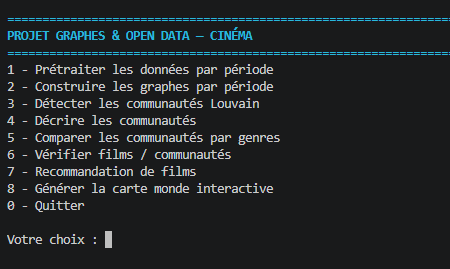
\includegraphics[width=0.75\textwidth]{annexes/menu.PNG}
    \caption{Menu principal du projet}
\end{figure}

\section{Prétraitement des données}

L’option 1 permet de filtrer les films selon les périodes étudiées : 1990--1999, 2000--2009 et 2010--2019. Cette étape génère un fichier CSV par période dans le dossier \texttt{data/processed}.

\begin{figure}[H]
    \centering
    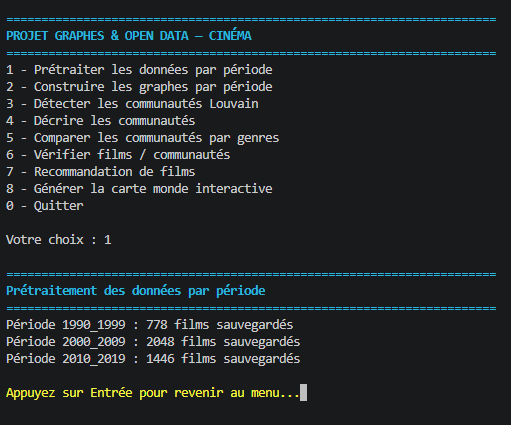
\includegraphics[width=0.85\textwidth]{annexes/option_1.PNG}
    \caption{Prétraitement des données par période}
\end{figure}

Cette étape confirme que les films sont bien répartis dans les trois périodes temporelles. Elle constitue la base de l’analyse temporelle du projet.

\section{Construction des graphes}

L’option 2 construit les graphes d’acteurs pour chaque période. Dans ces graphes, chaque nœud représente un acteur et chaque arête représente une collaboration entre deux acteurs ayant joué ensemble dans au moins un film.

L’utilisateur peut choisir le nombre d’acteurs à afficher dans la visualisation HTML (10 acteurs pour cet exemple). Cela permet de garder un graphe lisible tout en conservant les fichiers complets pour l’analyse.

\begin{figure}[H]
    \centering
    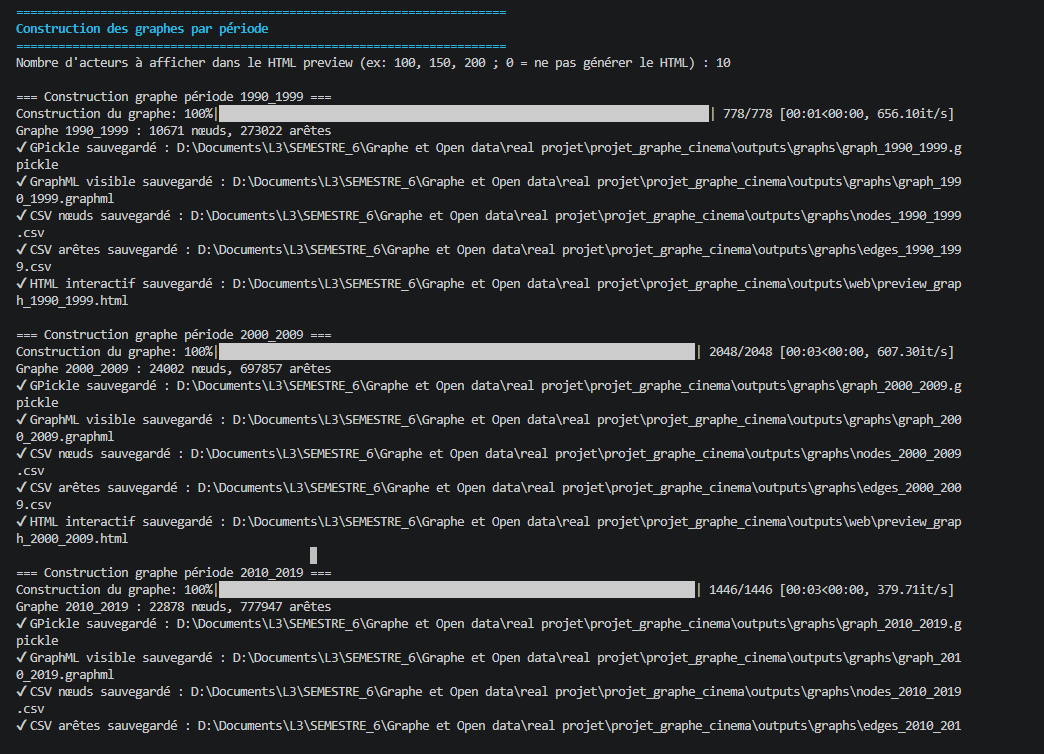
\includegraphics[width=0.95\textwidth]{annexes/option_2_menu.PNG}
    \caption{Construction des graphes par période depuis le menu}
\end{figure}

La capture suivante présente un exemple de graphe interactif généré avec un petit nombre d’acteurs. Les nœuds représentent les acteurs et les liens représentent les collaborations.

\begin{figure}[H]
    \centering
    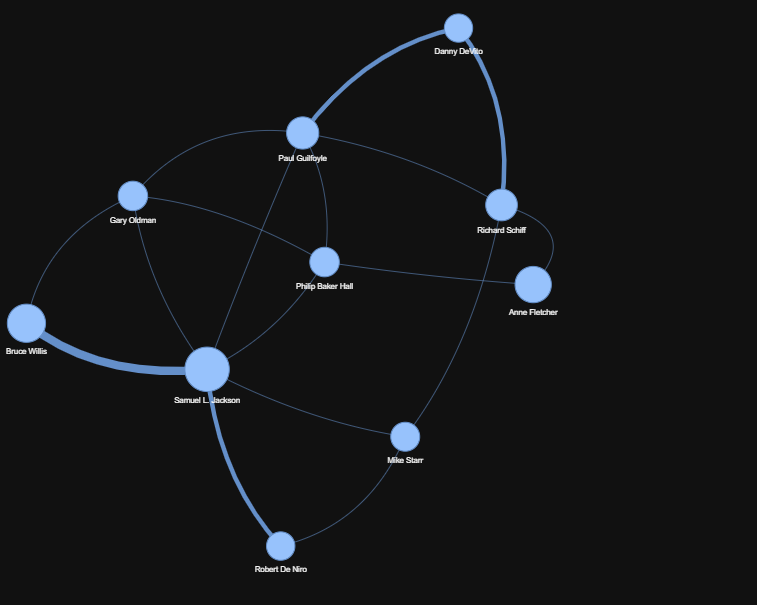
\includegraphics[width=0.70\textwidth]{annexes/option2.PNG}
    \caption{Exemple de graphe interactif généré}
\end{figure}

Dans la visualisation interactive, le survol d’un acteur affiche des informations détaillées : nom de l’acteur, période, degré total, degré visible dans le sous-graphe, collaborateurs visibles et films associés.

\begin{figure}[H]
    \centering
    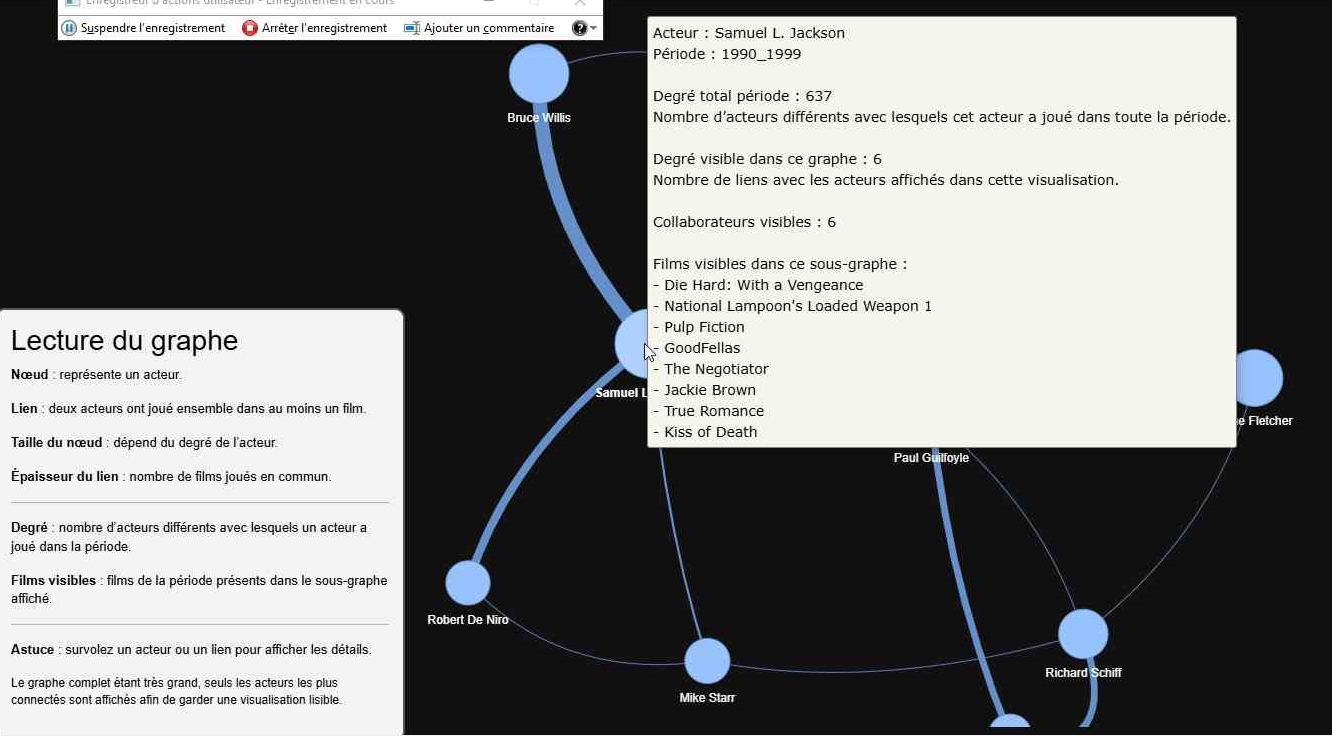
\includegraphics[width=1.1\textwidth]
    {annexes/option2_test_10_noeud.PNG}
    \caption{Informations affichées au survol d’un acteur}
\end{figure}

Le survol d’un lien affiche les deux acteurs reliés, le nombre de films en commun et le nom des films concernés. Cela permet de vérifier concrètement la signification des arêtes du graphe.

\begin{figure}[H]
    \centering
    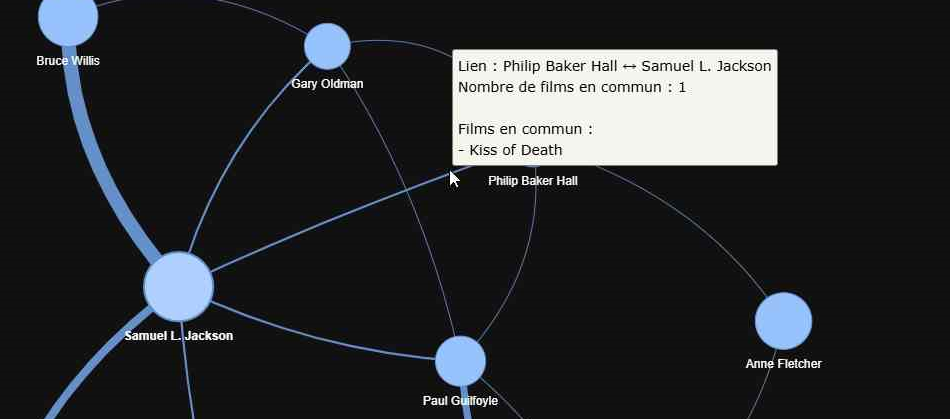
\includegraphics[width=0.95\textwidth]{annexes/option2_test_10_liens.PNG}
    \caption{Informations affichées au survol d’un lien}
\end{figure}

\section{Détection des communautés Louvain}

L’option 3 applique l’algorithme de Louvain aux graphes construits. Cette étape permet d’identifier des communautés d’acteurs, c’est-à-dire des groupes d’acteurs plus fortement connectés entre eux qu’avec le reste du réseau.

\begin{figure}[H]
    \centering
    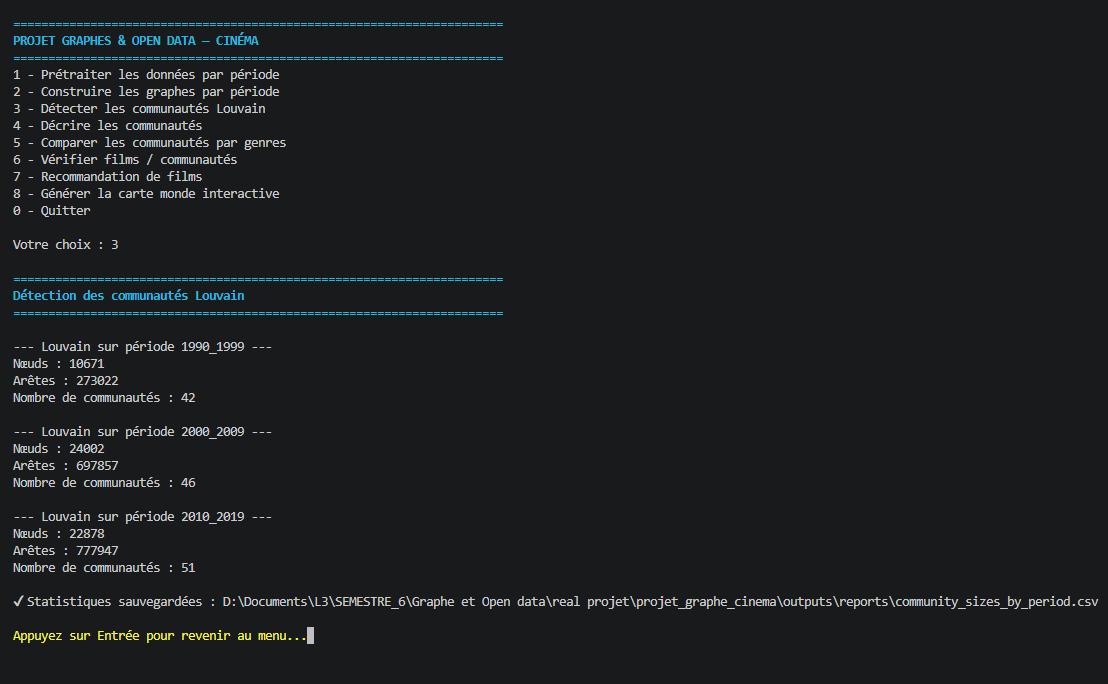
\includegraphics[width=1.0\textwidth]{annexes/option_3_menu.PNG}
    \caption{Détection des communautés Louvain par période}
\end{figure}

Le programme génère un fichier de synthèse indiquant, pour chaque période, les communautés détectées et leur taille.

\begin{figure}[H]
    \centering
    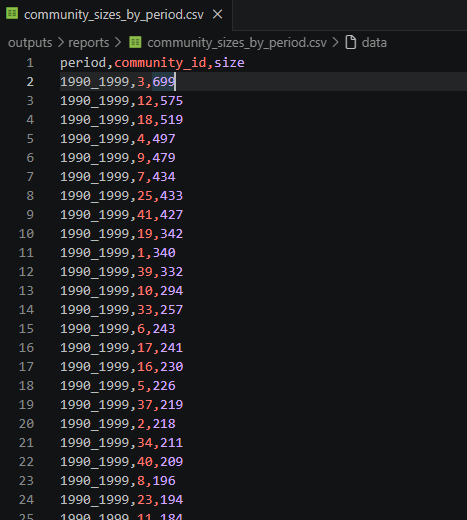
\includegraphics[width=0.42\textwidth]{annexes/option3_csv.PNG}
    \caption{Fichier CSV des tailles de communautés par période}
\end{figure}

\section{Description des communautés}

L’option 4 permet d’enrichir les communautés détectées. Les communautés Louvain n’ont pas de nom officiel dans le dataset : elles sont identifiées par des numéros. Le projet les décrit donc à partir des genres dominants, du nombre d’acteurs et du nombre de films associés.

\begin{figure}[H]
    \centering
    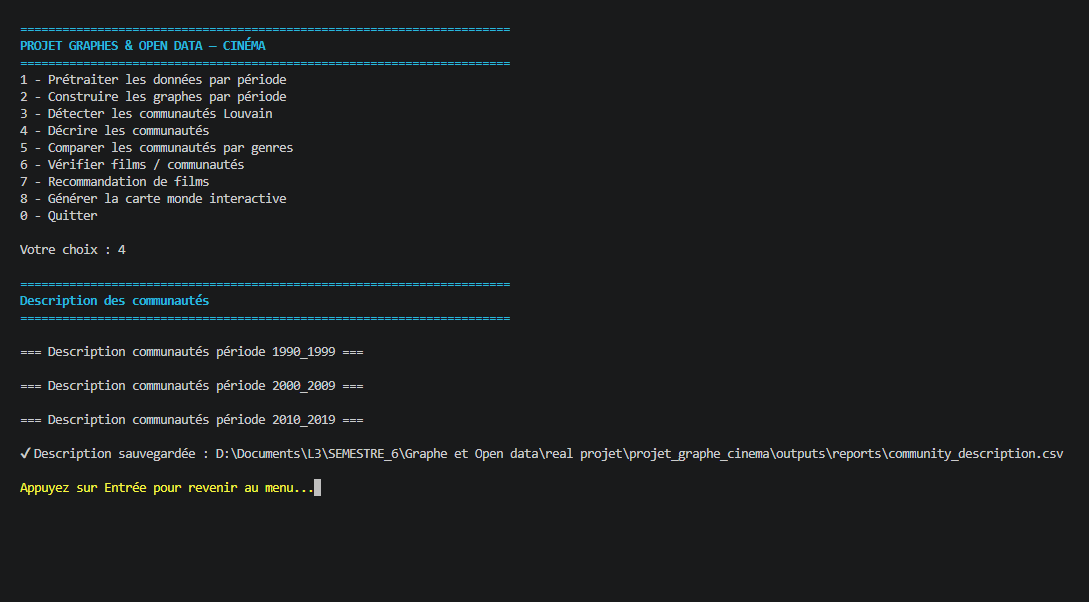
\includegraphics[width=1.02\textwidth]{annexes/option4_menu.PNG}
    \caption{Description des communautés détectées}
\end{figure}

Le fichier \texttt{community\_description.csv} contient une description synthétique de chaque communauté : période, identifiant de communauté, nombre d’acteurs, nombre de films et genres dominants.

\begin{figure}[H]
    \centering
    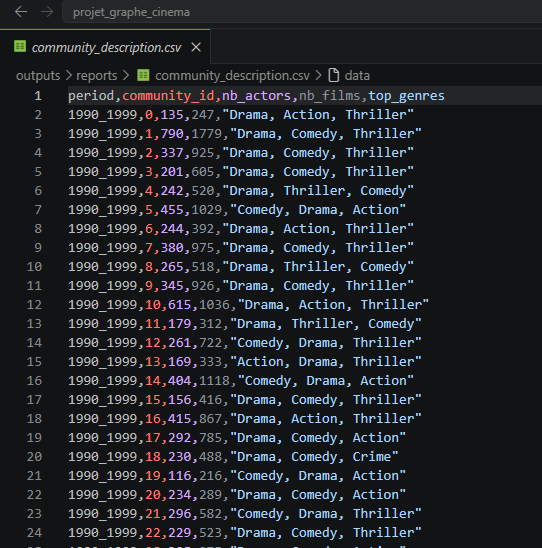
\includegraphics[width=0.5\textwidth]{annexes/option4_csv.PNG}
    \caption{Fichier de description des communautés}
\end{figure}

\section{Comparaison des communautés par genres}

L’option 5 compare les communautés selon leurs genres dominants. Cette étape permet de vérifier si certains genres structurent les communautés d’acteurs.

\begin{figure}[H]
    \centering
    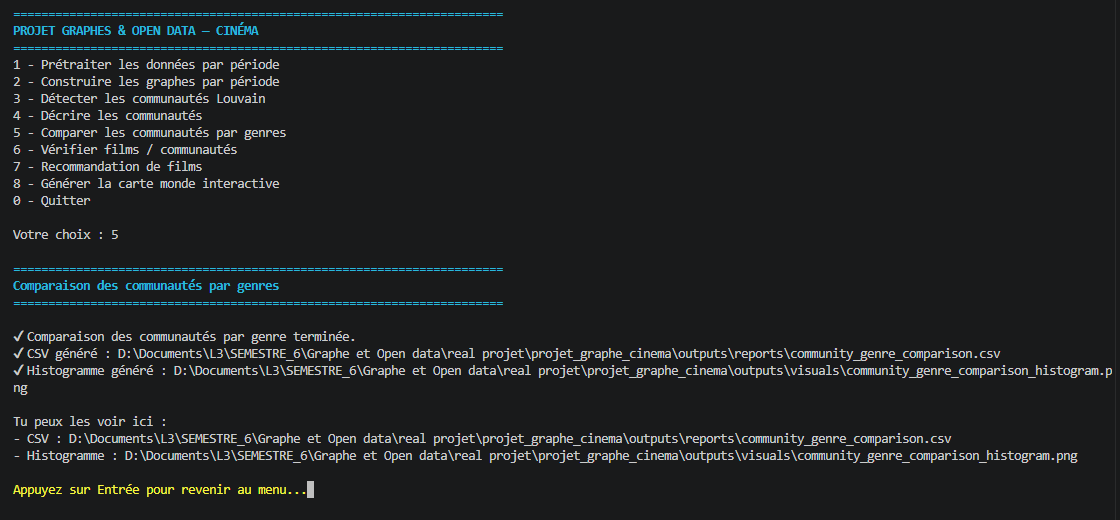
\includegraphics[width=1.1\textwidth]{annexes/option5_menu.PNG}
    \caption{Comparaison des communautés par genres depuis le menu}
\end{figure}

Le programme génère un fichier CSV contenant les genres dominants et le nombre de communautés correspondantes par période.

\begin{figure}[H]
    \centering
    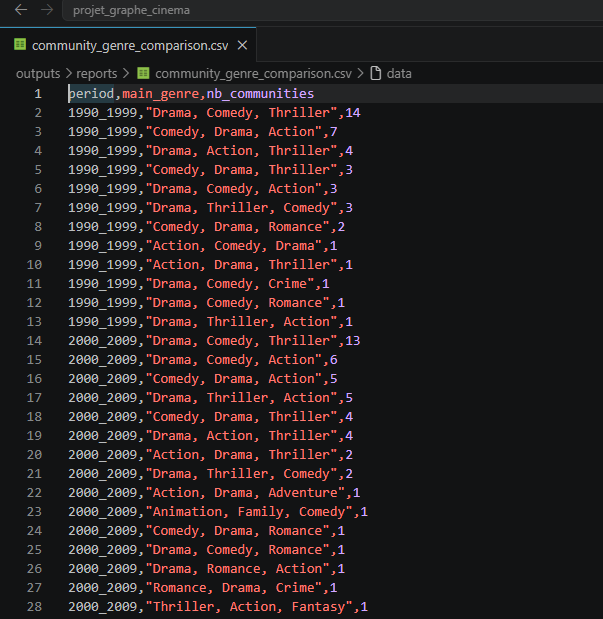
\includegraphics[width=0.60\textwidth]{annexes/option5_csv.PNG}
    \caption{Fichier CSV de comparaison des communautés par genres}
\end{figure}

Un histogramme est également généré afin de visualiser plus clairement la répartition des genres dominants selon les périodes.

\begin{figure}[H]
    \centering
    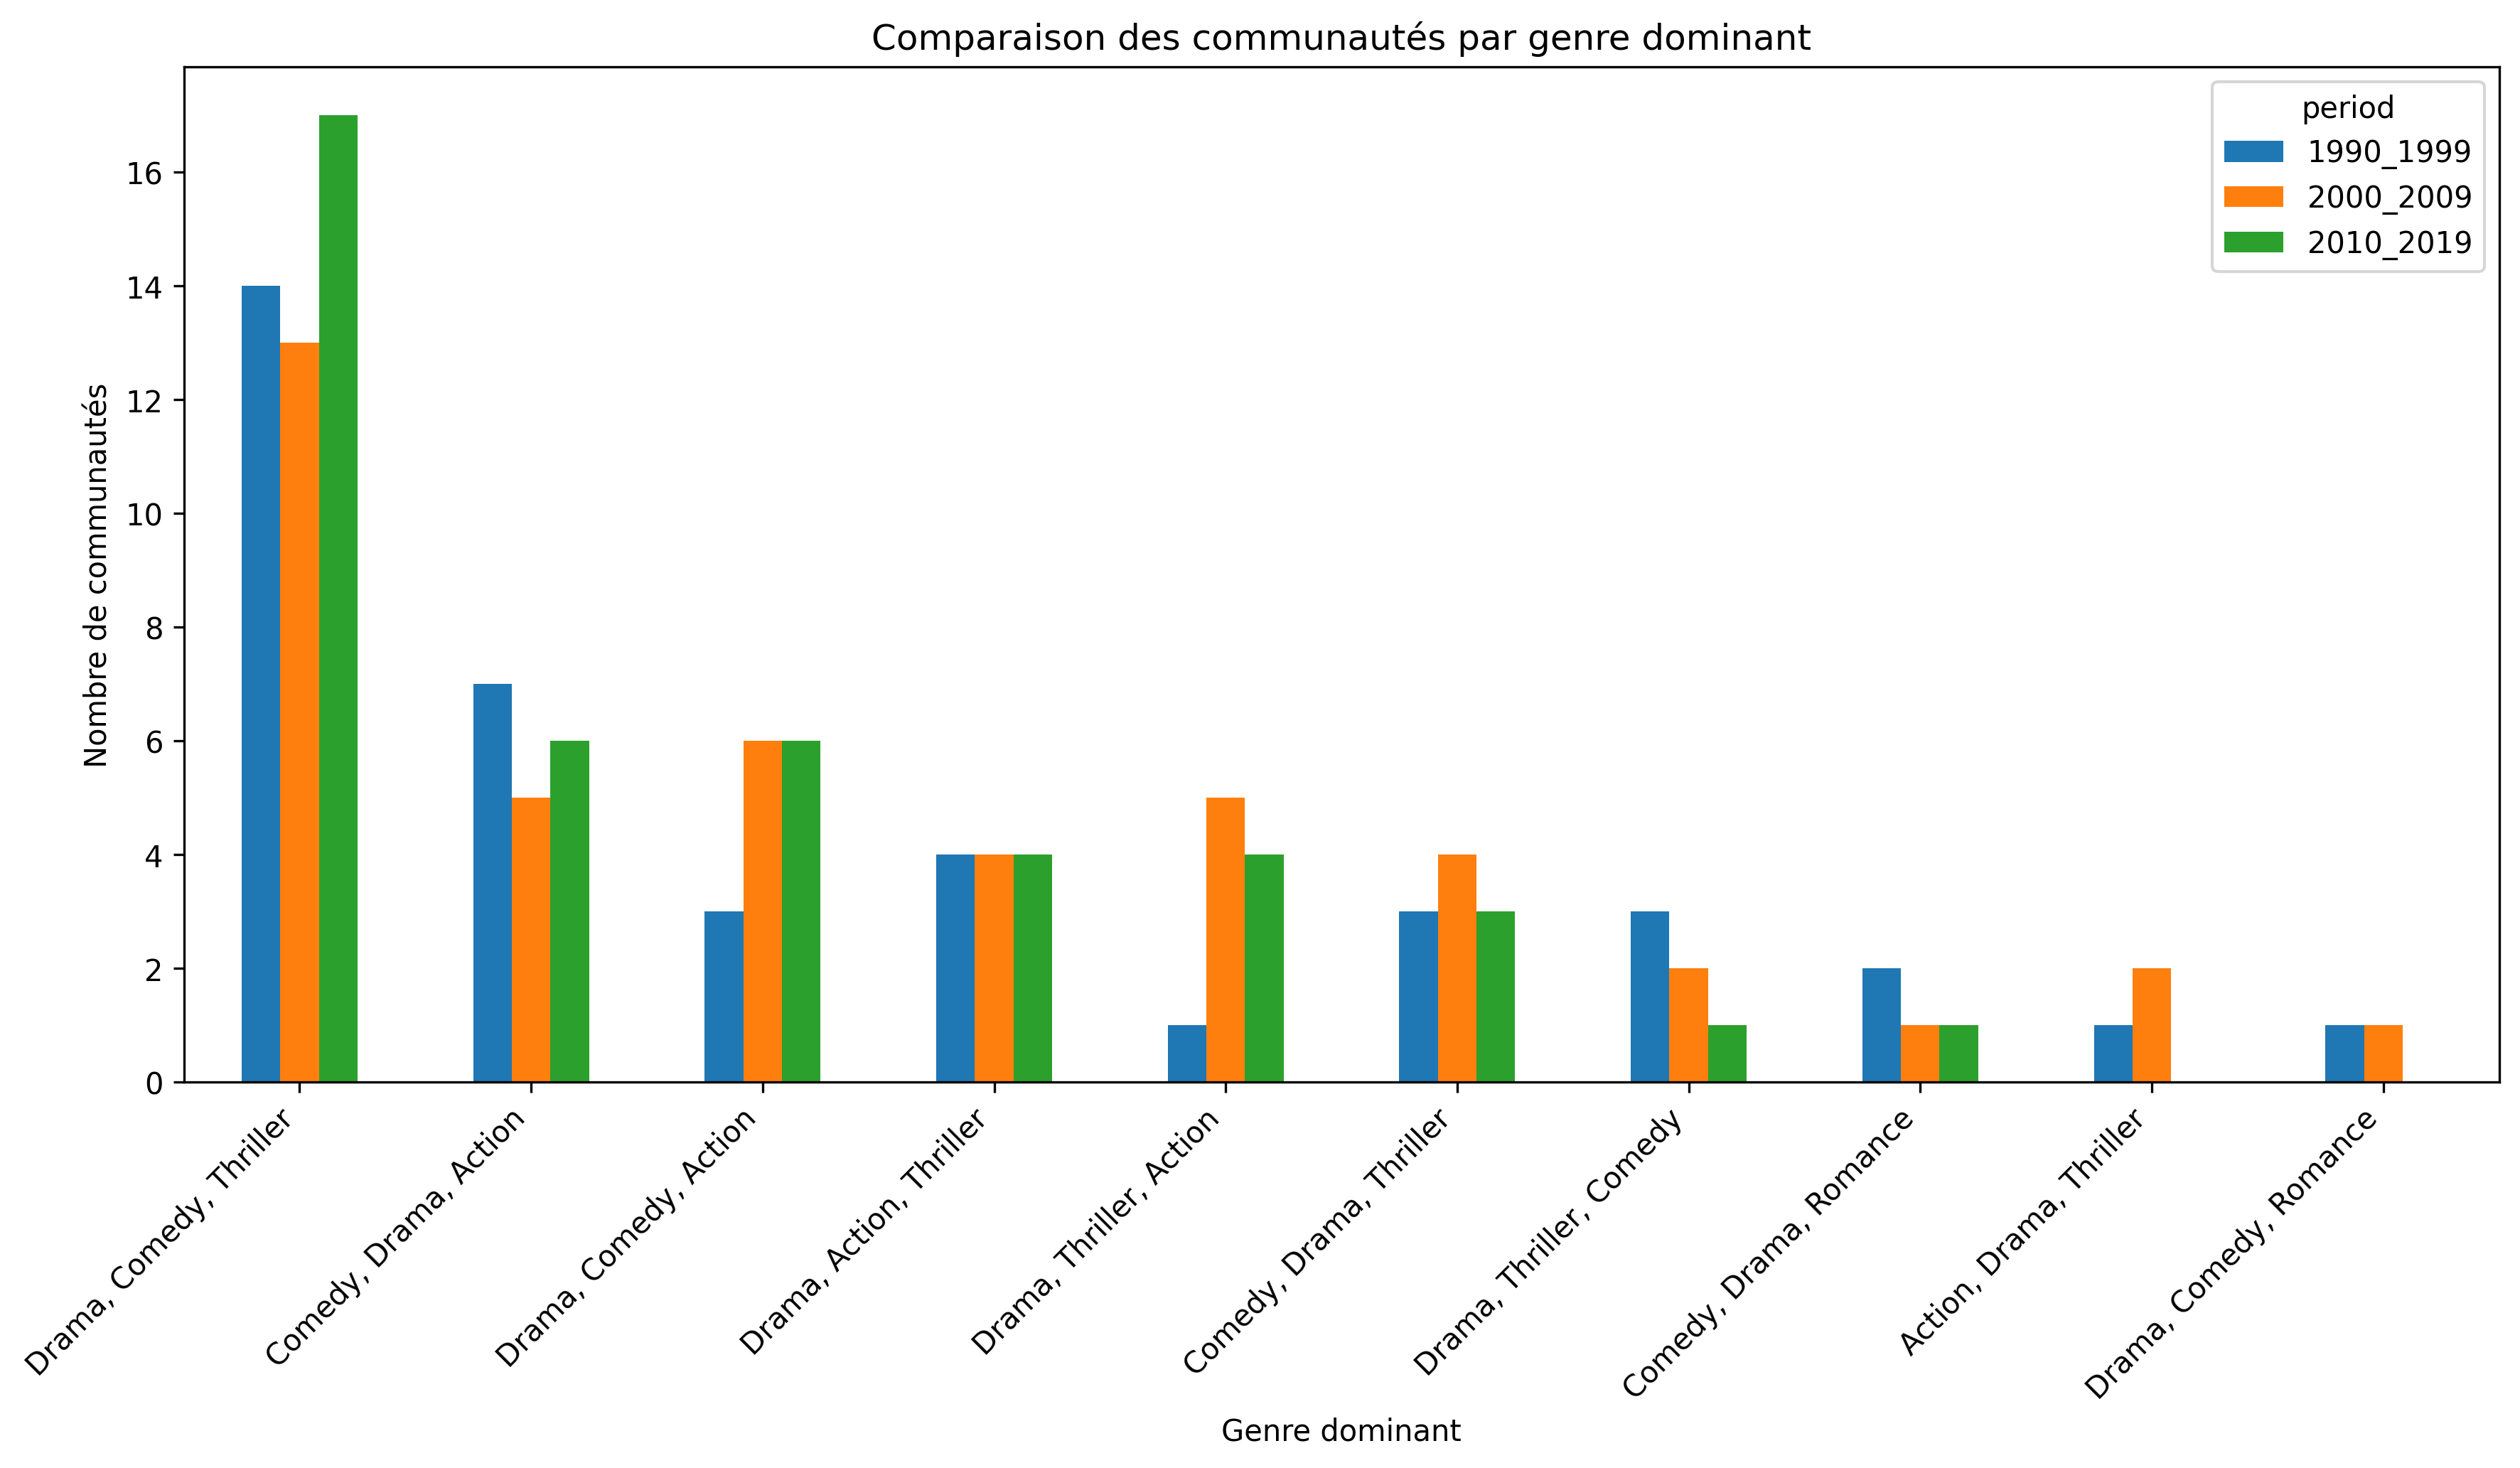
\includegraphics[width=0.9\textwidth]{annexes/option5_histogramme.png}
    \caption{Histogramme de comparaison des communautés par genre dominant}
\end{figure}

\section{Vérification films et communautés}

L’option 6 relie chaque film aux communautés de ses acteurs. Elle permet d’identifier les films cohérents avec une communauté et les films qui mélangent plusieurs communautés.

\begin{figure}[H]
    \centering
    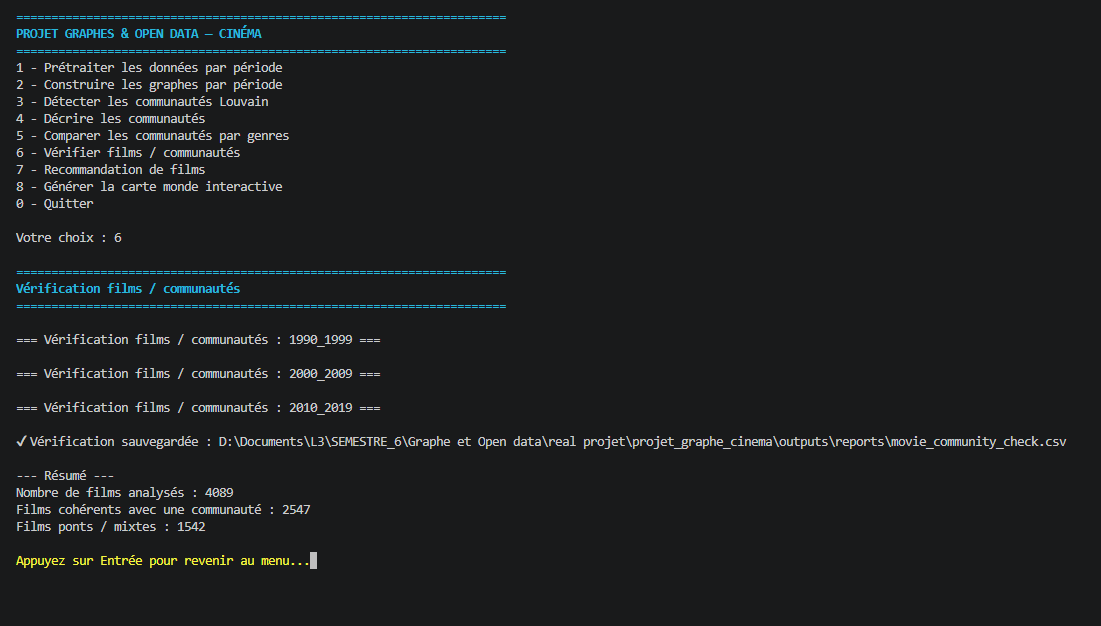
\includegraphics[width=1.0\textwidth]{annexes/option_6_menu.PNG}
    \caption{Vérification des films et des communautés}
\end{figure}

Le fichier généré contient, pour chaque film, la période, le titre, l’année, le nombre d’acteurs, le nombre de communautés présentes dans le film, la communauté dominante et la part de cette communauté dans la distribution.

\begin{figure}[H]
    \centering
    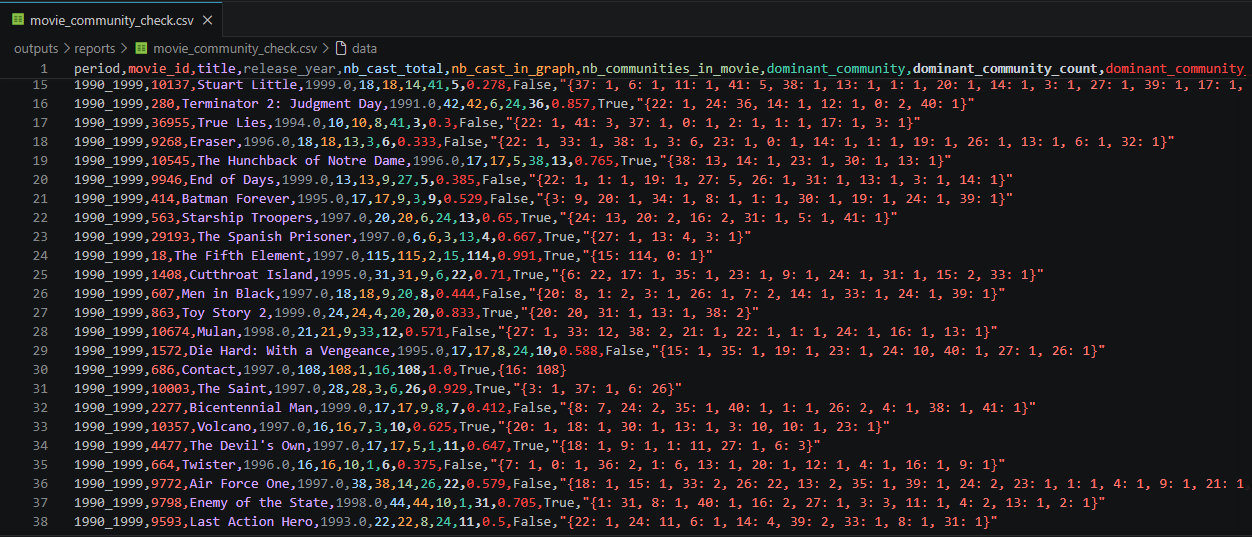
\includegraphics[width=1.1\textwidth]{annexes/option6_csv.PNG}
    \caption{Fichier de vérification films et communautés}
\end{figure}

Cette étape permet de distinguer les films principalement associés à une communauté des films-ponts, qui relient plusieurs groupes d’acteurs.

\section{Recommandation de films}

L’option 7 donne accès au module de recommandation. L’utilisateur peut recommander des films par genre, par acteur ou par communauté. Une option permet également de générer des exemples de fichiers CSV.

\begin{figure}[H]
    \centering
    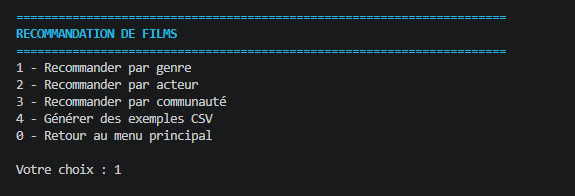
\includegraphics[width=0.98\textwidth]{annexes/option_7.PNG}
    \caption{Menu de recommandation de films}
\end{figure}

\subsection{Recommandation par genre}

Lorsque l’utilisateur choisit une recommandation par genre, le programme affiche les genres disponibles dans le dataset. L’utilisateur sélectionne ensuite un genre par numéro.

\begin{figure}[H]
    \centering
    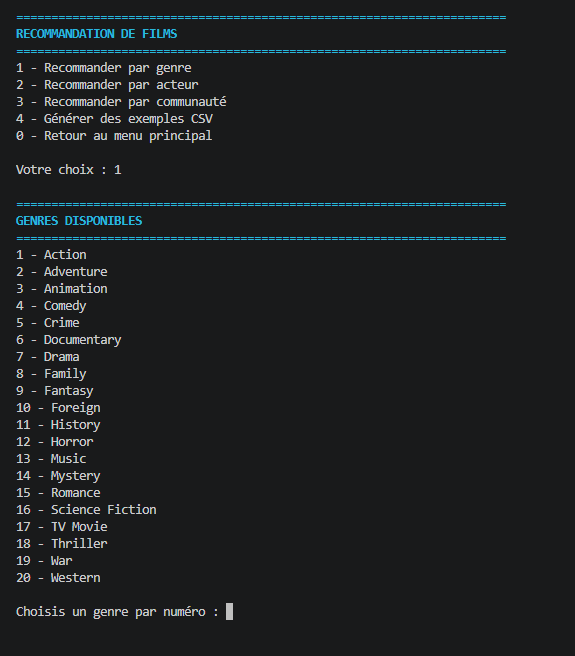
\includegraphics[width=0.65\textwidth]{annexes/option_7_menu.PNG}
    \caption{Liste des genres disponibles}
\end{figure}

La capture suivante montre un exemple de recommandation par genre. L’utilisateur choisit un genre, une période et le nombre de recommandations souhaitées. Le programme affiche ensuite les films correspondants, avec leur année, leurs genres, leur note moyenne, leur popularité et leur période.

\begin{figure}[H]
    \centering
    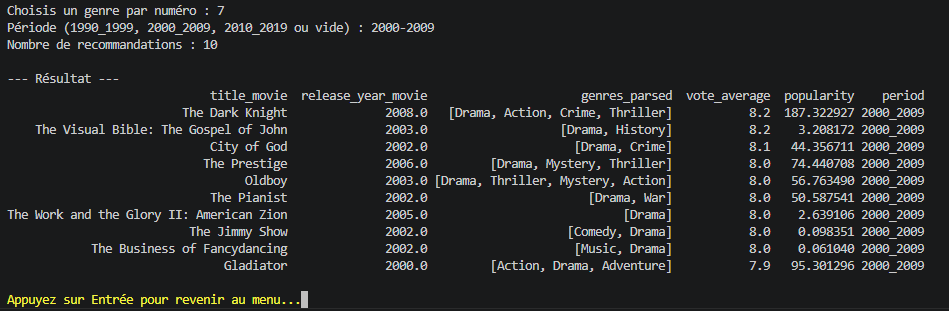
\includegraphics[width=1.0\textwidth]{annexes/option_7_menu_1.PNG}
    \caption{Exemple de recommandation par genre}
\end{figure}

\subsection{Recommandation par acteur}

Le deuxième mode permet de rechercher un acteur. Le programme propose les acteurs trouvés dans la base, puis l’utilisateur choisit celui qui l’intéresse.

\begin{figure}[H]
    \centering
    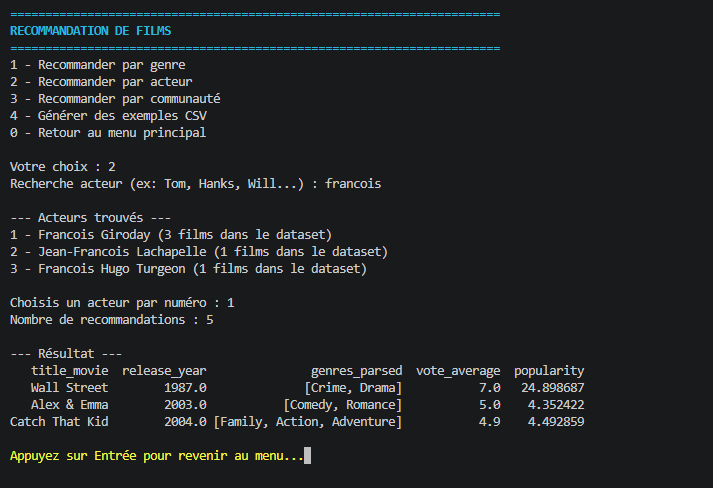
\includegraphics[width=1.0\textwidth]{annexes/option_7_menu_2.PNG}
    \caption{Recherche d’un acteur dans la base}
\end{figure}

Après sélection de l’acteur, le programme retourne des films associés à cet acteur. Cette fonctionnalité permet à l’utilisateur d’explorer le dataset à partir d’un nom d’acteur.

\subsection{Recommandation par communauté}

Le troisième mode permet de recommander des films à partir d’une communauté dominante. Comme l’utilisateur ne connaît pas directement les identifiants des communautés, le programme affiche une liste descriptive des communautés disponibles.

\begin{figure}[H]
    \centering
    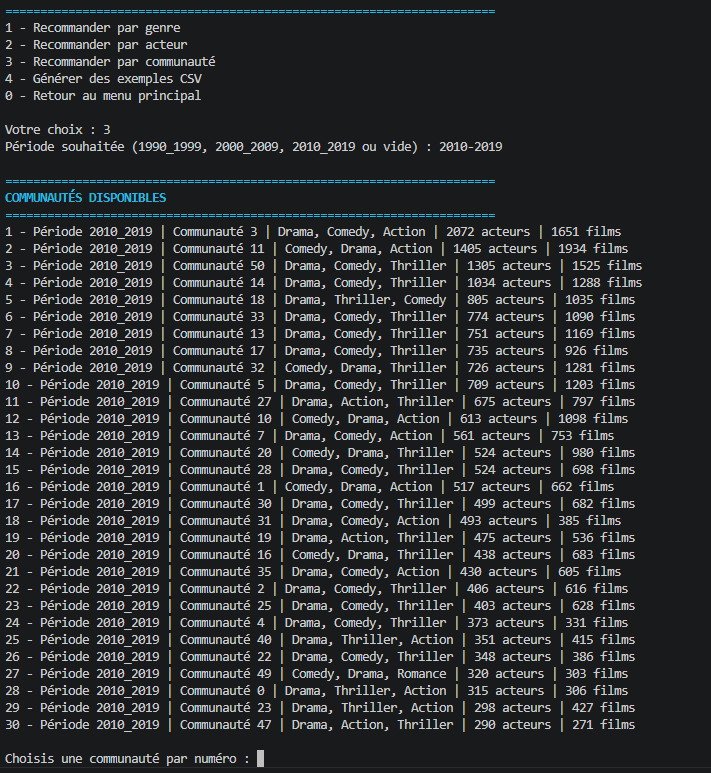
\includegraphics[width=0.8\textwidth]{annexes/option_7_menu_3_1.PNG}
    \caption{Liste des communautés disponibles pour la recommandation}
\end{figure}

Après le choix d’une communauté, le programme recommande des films associés à cette communauté dominante.

\begin{figure}[H]
    \centering
    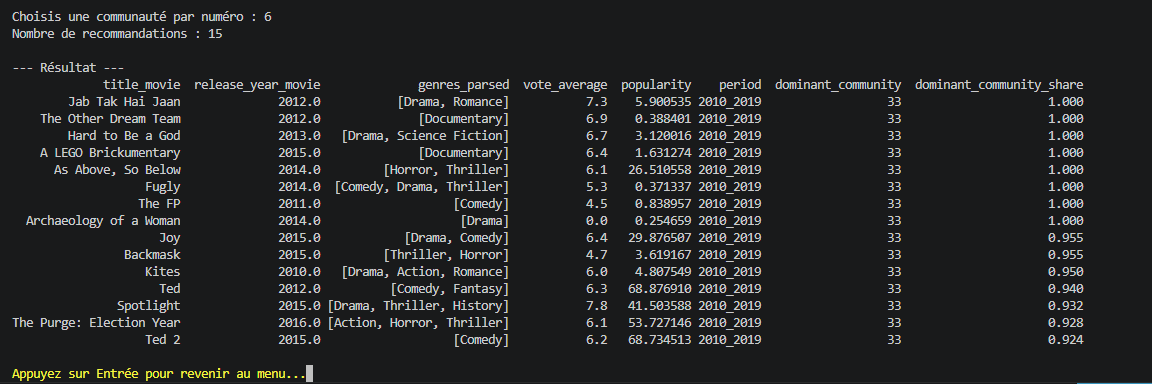
\includegraphics[width=1.1\textwidth]{annexes/option_7_menu_3_2.PNG}
    \caption{Résultat d’une recommandation par communauté}
\end{figure}

\subsection{Générer des exemples CSV}
L’option de génération d’exemples permet de créer automatiquement des fichiers CSV de recommandations.

\begin{figure}[H]
    \centering
    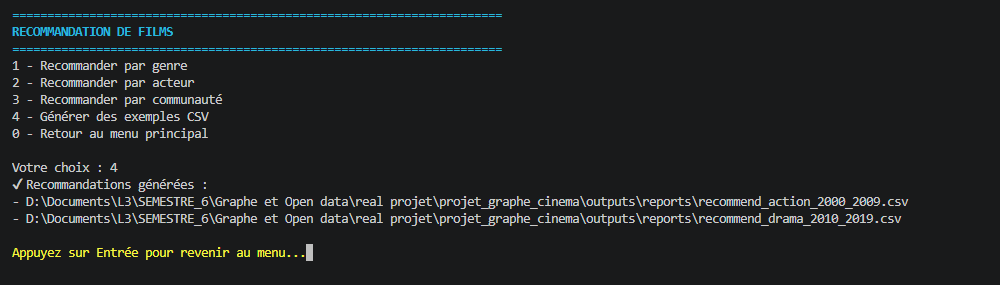
\includegraphics[width=1.1\textwidth]{annexes/option_7_menu_4.PNG}
    \caption{Génération automatique des fichiers CSV de recommandation}
\end{figure}

Exemple de fichier généré pour une recommandation de films d’action sur la période 2000--2009.

\begin{figure}[H]
    \centering
    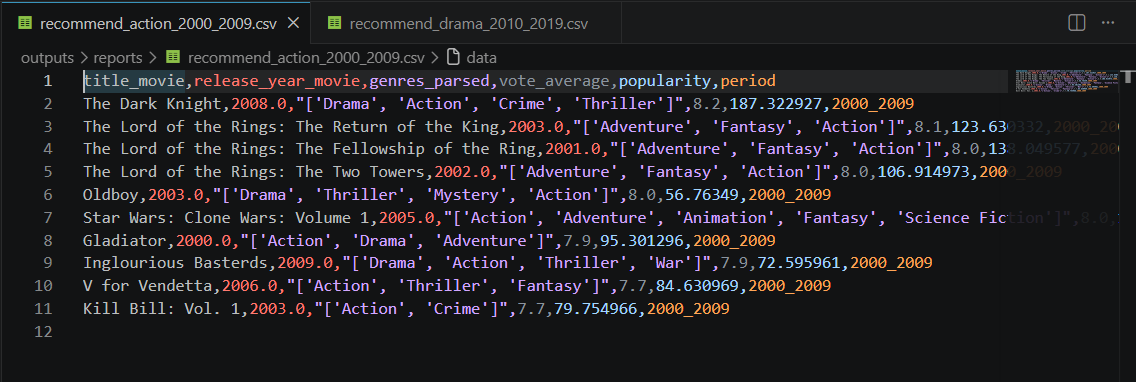
\includegraphics[width=0.85\textwidth]{annexes/option7_4_csv_2_action.PNG}
    \caption{Exemple de fichier CSV de recommandation Action 2000--2009}
\end{figure}

Exemple de fichier généré pour une recommandation de films dramatiques sur la période 2010--2019.

\begin{figure}[H]
    \centering
    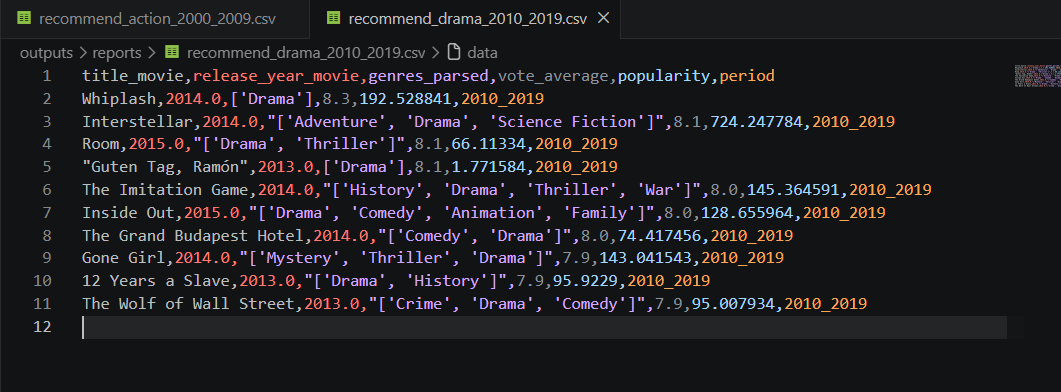
\includegraphics[width=0.85\textwidth]{annexes/option7_4_csv_1.PNG}
    \caption{Exemple de fichier CSV de recommandation Drama 2010--2019}
\end{figure}

\section{Carte monde interactive}

L’option 8 permet de générer une carte monde interactive. Les acteurs sont positionnés selon le pays dominant de production des films dans lesquels ils apparaissent. Cette information est une approximation, car le dataset ne contient pas le lieu de naissance des acteurs.

L’utilisateur peut générer une carte pour une seule période.

\begin{figure}[H]
    \centering
    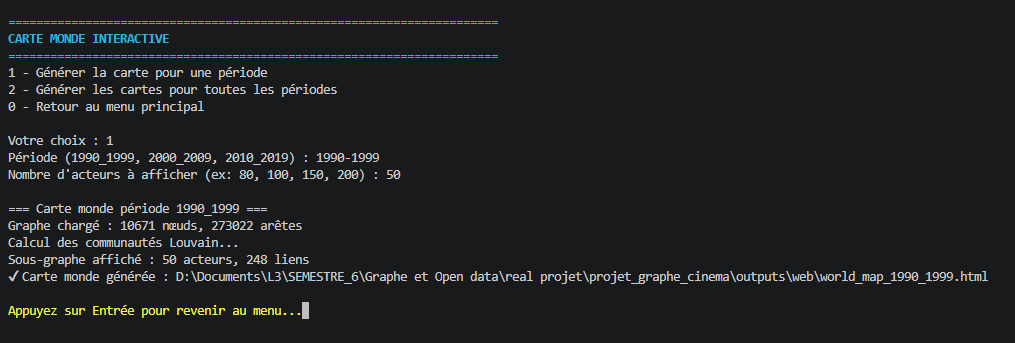
\includegraphics[width=0.95\textwidth]{annexes/option_8_menu_1.PNG}
    \caption{Génération d’une carte monde pour une période}
\end{figure}

Il peut également générer les cartes pour toutes les périodes.

\begin{figure}[H]
    \centering
    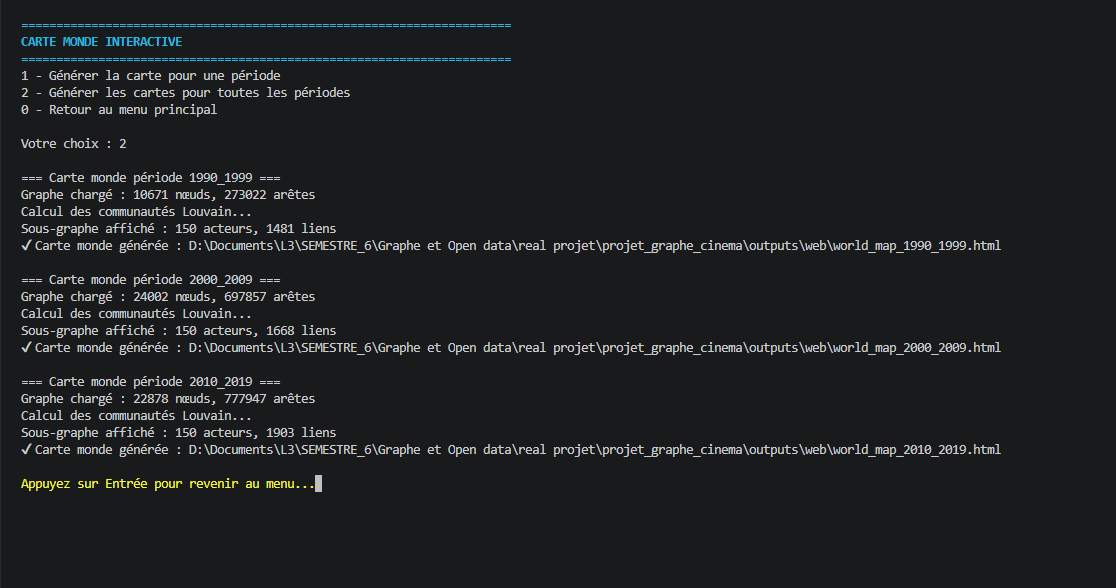
\includegraphics[width=0.95\textwidth]{annexes/option_8_menu_2.PNG}
    \caption{Génération des cartes monde pour toutes les périodes}
\end{figure}

La carte affiche les acteurs sous forme de points. La couleur représente la communauté Louvain, la taille représente le degré total de l’acteur dans la période, et les liens jaunes représentent les collaborations affichées sur la carte.

\begin{figure}[H]
    \centering
    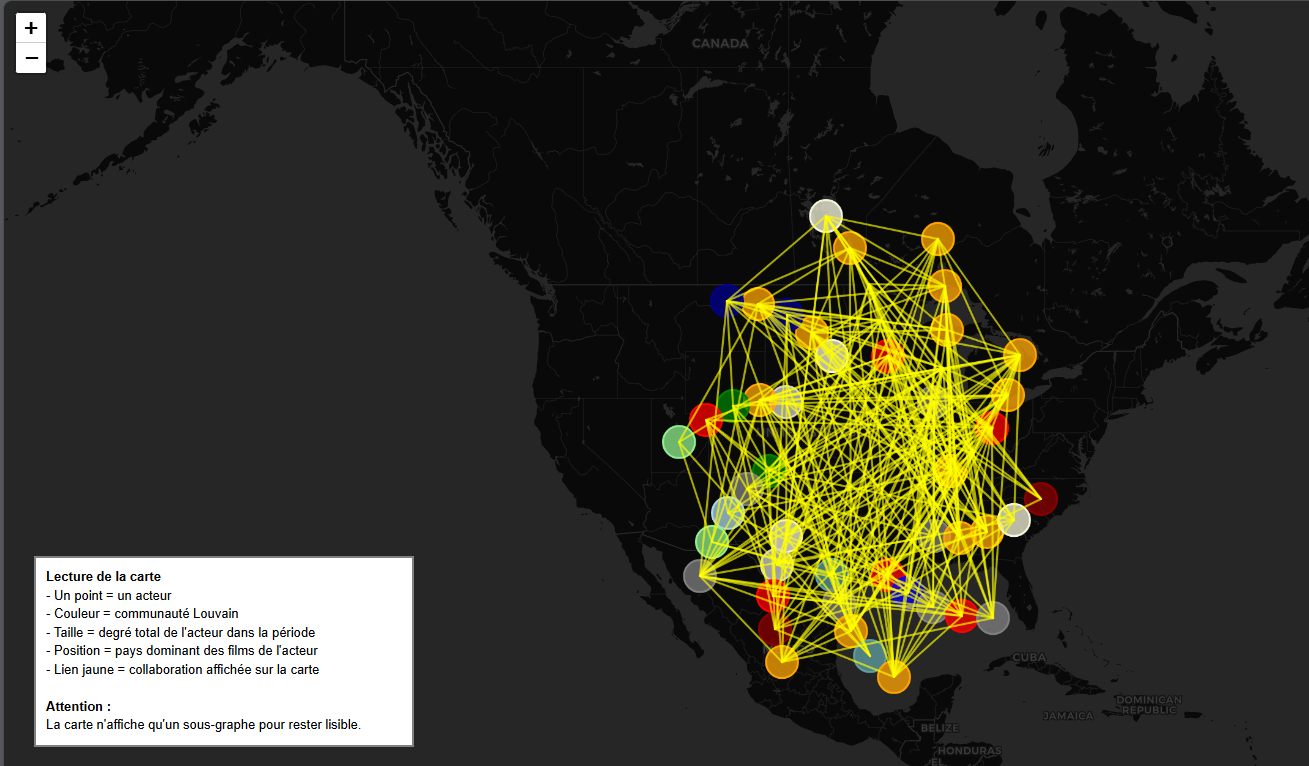
\includegraphics[width=0.8\textwidth]{annexes/option8_1_world_map.PNG}
    \caption{Carte monde interactive générée pour une période}
\end{figure}

Lorsqu’un acteur est sélectionné, une infobulle affiche ses informations : communauté, degré total, degré dans le sous-graphe, pays dominant, genres dominants et films dans la période.

\begin{figure}[H]
    \centering
    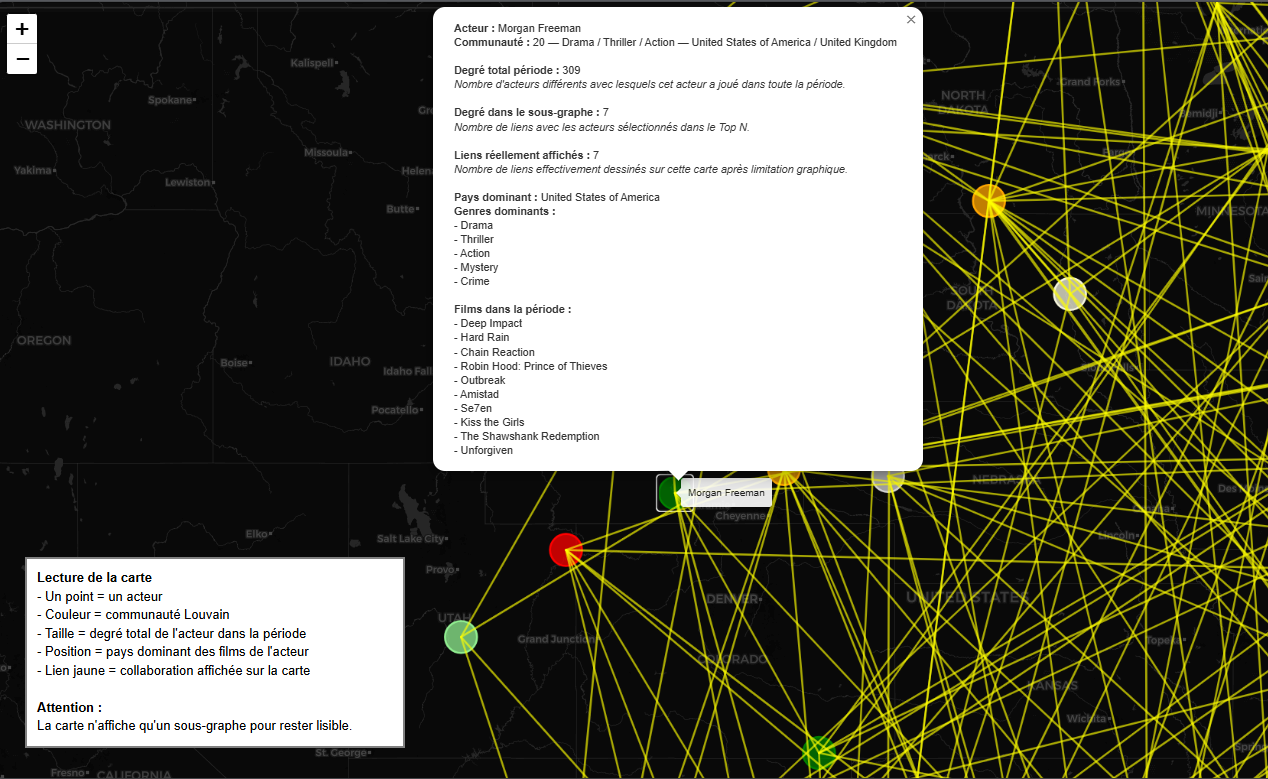
\includegraphics[width=1.1\textwidth]{annexes/option8_1_world_map_arrete.PNG}
    \caption{Informations affichées sur un acteur dans la carte interactive}
\end{figure}

Le survol ou le clic sur un lien permet d’afficher les deux acteurs reliés, le nombre de films en commun et les noms des films concernés.

\begin{figure}[H]
    \centering
    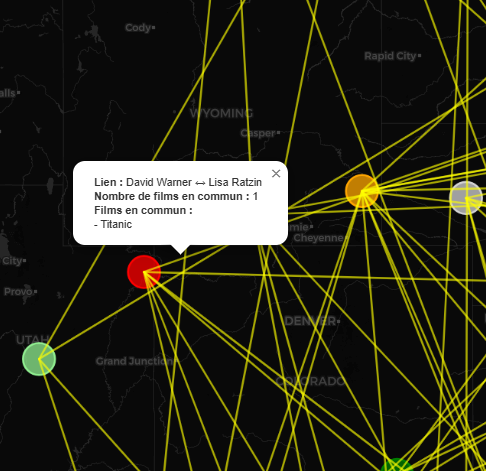
\includegraphics[width=0.6\textwidth]{annexes/option8_1_world_map_lien.PNG}
    \caption{Informations affichées sur un lien de collaboration dans la carte}
\end{figure}

La capture suivante montre une carte plus dense générée avec davantage d’acteurs. Elle illustre l’importance de limiter le nombre d’acteurs affichés afin de conserver une visualisation lisible.

\begin{figure}[H]
    \centering
    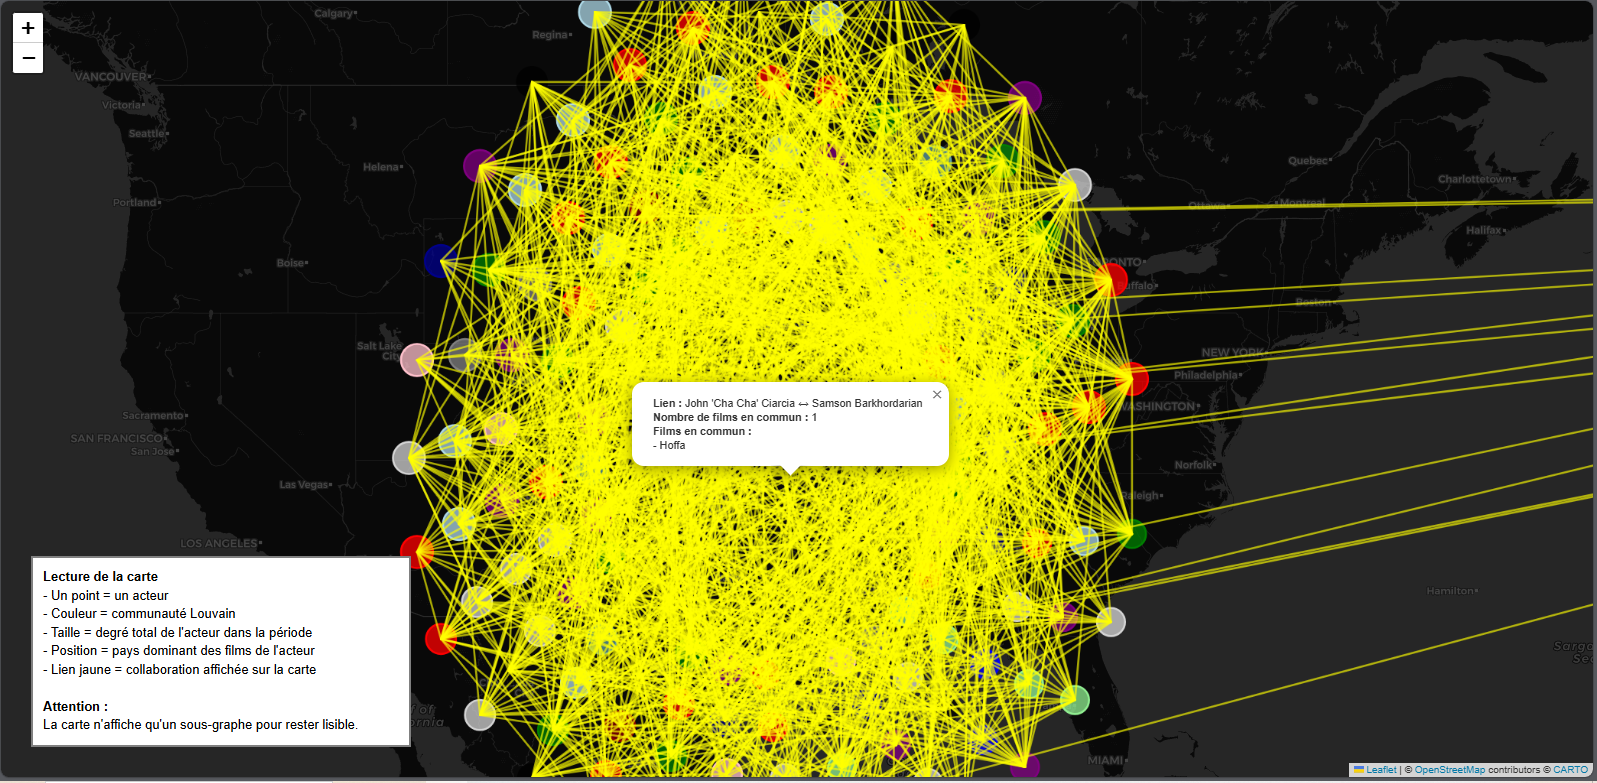
\includegraphics[width=1.1\textwidth]{annexes/option8_2_world_map.PNG}
    \caption{Carte monde interactive avec un nombre plus important d’acteurs}
\end{figure}

\section{Fichiers générés par le projet}

Le projet génère plusieurs types de fichiers afin de rendre les résultats exploitables.

\subsection{Dossier \texttt{data/processed}}

Ce dossier contient les fichiers CSV filtrés par période :

\begin{itemize}
    \item \texttt{movies\_1990\_1999.csv}
    \item \texttt{movies\_2000\_2009.csv}
    \item \texttt{movies\_2010\_2019.csv}
\end{itemize}

\subsection{Dossier \texttt{outputs/graphs}}

Ce dossier contient les graphes et les fichiers associés :

\begin{itemize}
    \item fichiers \texttt{.gpickle} utilisés par Python ;
    \item fichiers \texttt{.graphml} exploitables dans Gephi ;
    \item fichiers CSV des nœuds ;
    \item fichiers CSV des arêtes.
\end{itemize}

\subsection{Dossier \texttt{outputs/reports}}

Ce dossier contient les fichiers de résultats :

\begin{itemize}
    \item \texttt{community\_sizes\_by\_period.csv}
    \item \texttt{community\_description.csv}
    \item \texttt{community\_genre\_comparison.csv}
    \item \texttt{movie\_community\_check.csv}
    \item \texttt{recommend\_action\_2000\_2009.csv}
    \item \texttt{recommend\_drama\_2010\_2019.csv}
\end{itemize}

\subsection{Dossier \texttt{outputs/visuals}}

Ce dossier contient les graphiques générés, notamment :

\begin{itemize}
    \item \texttt{community\_genre\_comparison\_histogram.png}
\end{itemize}

\subsection{Dossier \texttt{outputs/web}}

Ce dossier contient les visualisations interactives :

\begin{itemize}
    \item \texttt{preview\_graph\_1990\_1999.html}
    \item \texttt{preview\_graph\_2000\_2009.html}
    \item \texttt{preview\_graph\_2010\_2019.html}
    \item \texttt{world\_map\_1990\_1999.html}
    \item \texttt{world\_map\_2000\_2009.html}
    \item \texttt{world\_map\_2010\_2019.html}
\end{itemize}
\end{document}